\documentclass[12pt]{article}
\title{Time Series Analysis - Energy Consumption}
\date{April 8, 2018}
\author{Bach Quang Minh - MS Candidate - John Von Neumann Institute}
\usepackage{hyperref}
\usepackage{graphicx}
\usepackage{float}
\usepackage{subcaption}
\usepackage{amsmath}
\usepackage{siunitx}

\begin{document}
\maketitle
\pagenumbering{gobble}

\newpage
\tableofcontents

\newpage
\pagenumbering{arabic}

\section{Data description}
\paragraph{}
The data set shows different measures of a particular household, including temperature, humidity conditions, weather conditions and energy consumption.
The data set is at 10 min for about 4.5 months, containing 19736 data points and 30 attributes in total.
Therefore, no time-interval adjustments are needed.
The outcome of interest is the ‘Appliances’ column, which contains the energy consumption of the house.
For the analysis task, a sample of 10 days from 1/12/2016 00:00 to 1/21/2016 23:50 is extracted from the data, keeping only the "date" and the "Appliances" columns.
The sample contains 1440 data points which is used for the fitting process. 
The forecast is made for the next 2 hours, projecting 12 data points ahead.

\paragraph{}
The data can be downloaded 
\href{https://archive.ics.uci.edu/ml/datasets/Appliances+energy+prediction#}{here}.

\paragraph{}
The following figure gives an overall look of the data set. 
\begin{figure}[H]
  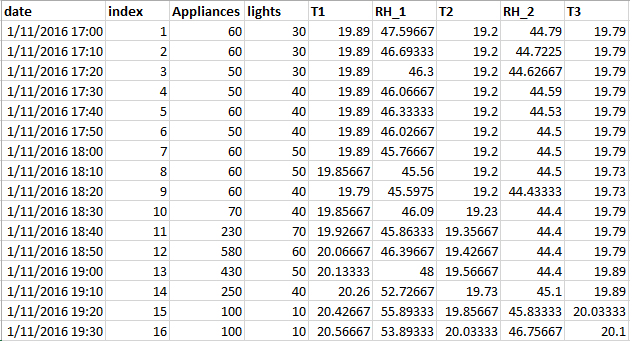
\includegraphics[width=\linewidth]{figure1.png}
  \caption{This is a snapshot of the data. The figure only shows 9 out of 30 attributes.}
  \label{fig:figure1}
\end{figure}

\section{Data exploration}
\paragraph{}
First, the "Appliances" is graphed as a time series.
\begin{figure}[H]
  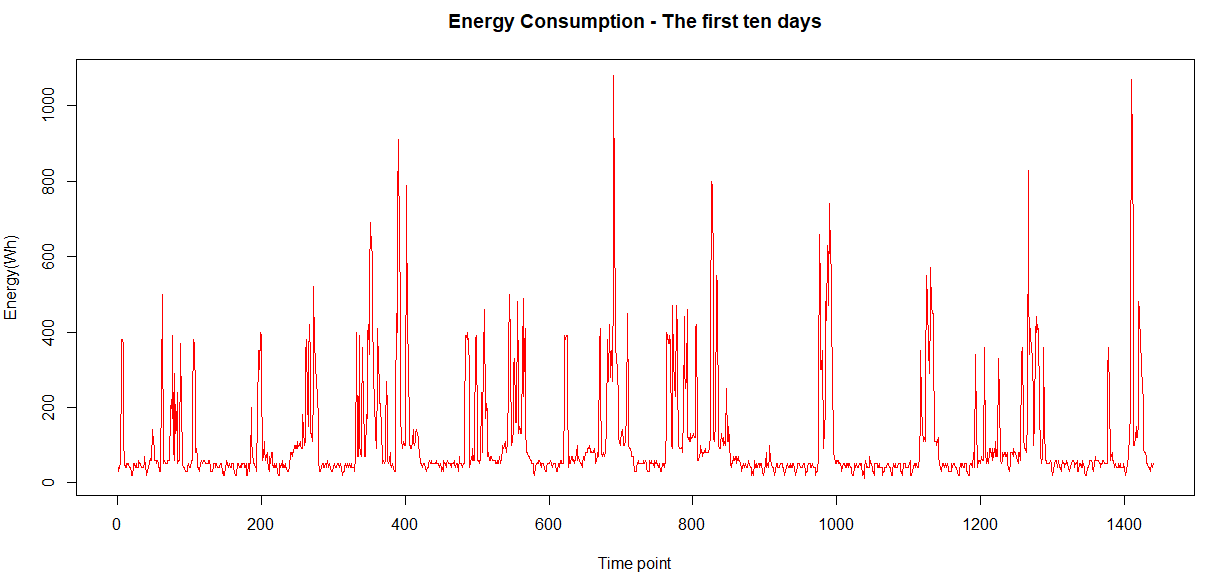
\includegraphics[width=\linewidth]{figure2.png}
  \caption{First look at the time series.}
  \label{fig:figure2}
\end{figure}

\paragraph{}
As can be seen, there is a high volatility in the energy consumption over time. There are some points where the energy level gets very high, meanwhile some durations see significantly low levels of energy. This could be due to the family members' activities. There is a slight pattern of seasonality. The following graph is made to investigate seasonality in the time series Figure ~\ref{fig:figure3}.
\begin{figure}[H]
  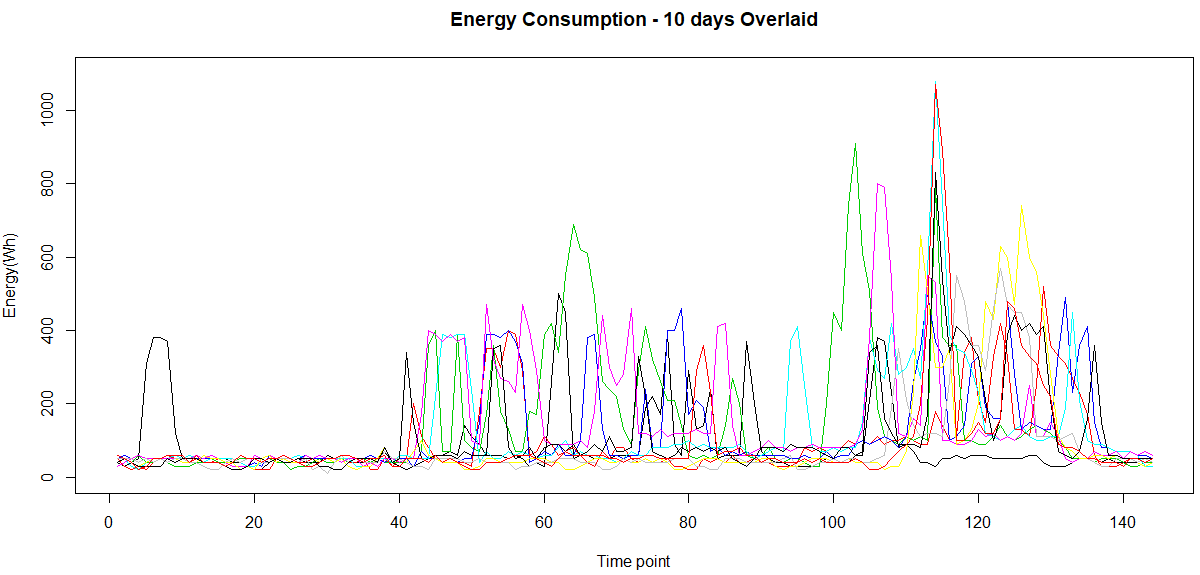
\includegraphics[width=\linewidth]{figure3.png}
  \caption{Each color represents one day's energy series.}
  \label{fig:figure3}
\end{figure}

\paragraph{}
Generally, a pattern in energy consumption can be seen from the graph. From the first 6 hours of a day, the consumption is quite low, fluctuating around 50Wh although an unusual event can be seen in day 1, creating a hump of 400Wh at around 1:30am (the black line). From 6:00am to around 3:30pm, a handful of days see high levels of energy consumption, meanwhile, some other days remain the same energy levels as those of the first 6 hours. After that energy levels back to around 50 Wh, then quickly jumps high, peaking at around 9:00pm. The consumption is quite high generally from 5:30pm to 11:00pm, then lowers back to around 50Wh.

\paragraph{}
To reduce the variability in the variance, the log10 transformation is  applied to the data, producing a quite stationary-in-mean series Figure ~\ref{fig:figure4}.
\begin{figure}[H]
  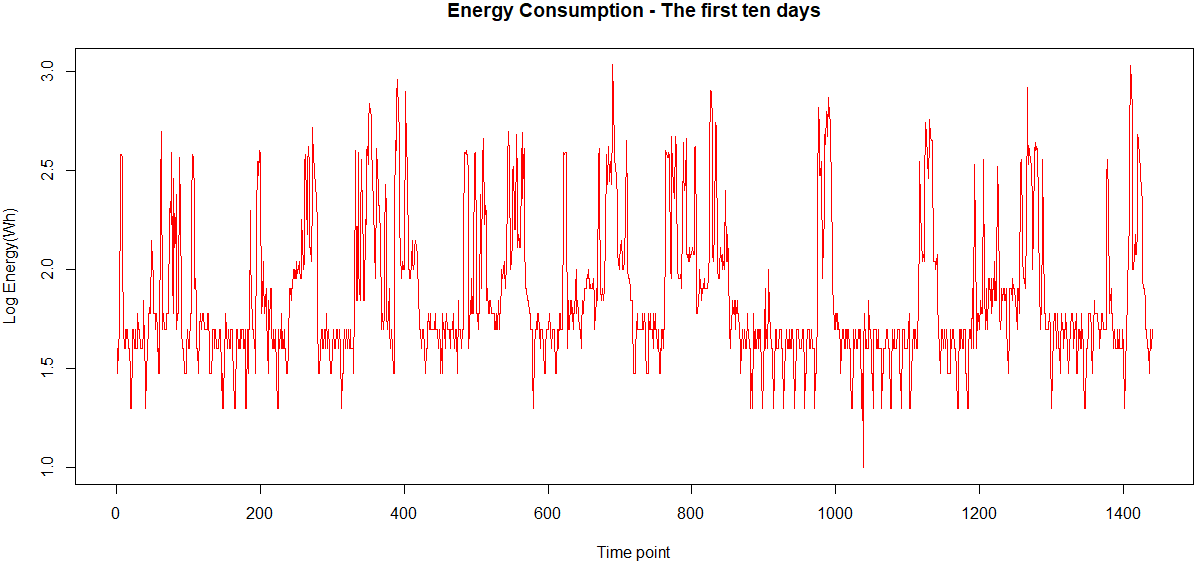
\includegraphics[width=\linewidth]{figure4.png}
  \caption{The time series in log base 10 scale. The series look quite stationary in mean and the variance is more stable}
  \label{fig:figure4}
\end{figure}

\paragraph{}
Further stationary analysis can be done by checking the acf and the pacf of the log series Figure ~\ref{fig:figure5}. Notice that the waving patterns in the acf plot, together with the fact that significant numbers of lags show high autocorrelation, give evidence against stationarity in the series, although the pacf show a quite good shape. 
\begin{figure}[H]
  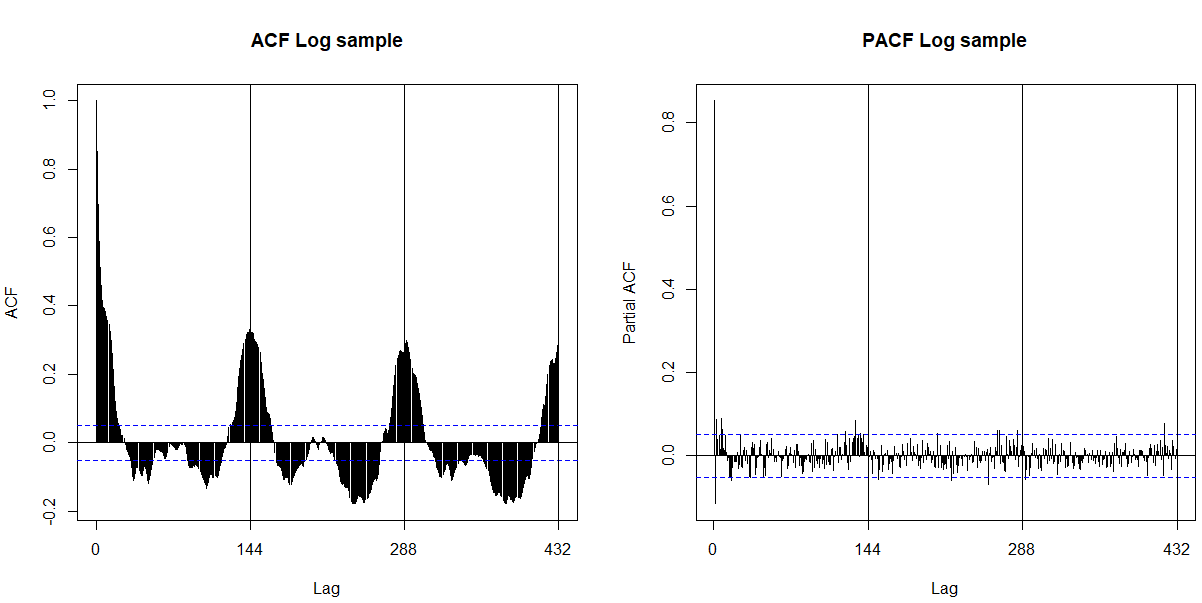
\includegraphics[width=\linewidth]{figure5.png}
  \caption{The acf plot does not show strong evidence of stationarity}
  \label{fig:figure5}
\end{figure}

\paragraph{}
The first order difference of the log series is taken at lag 1 in attempting to stationarize the series. Figure ~\ref{fig:figure6}  shows that the difference series looks stationary in mean 0. However, the variance varies unpredictably over time. Again, acf and pacf plots are checked for further conclusion.
\begin{figure}[H]
  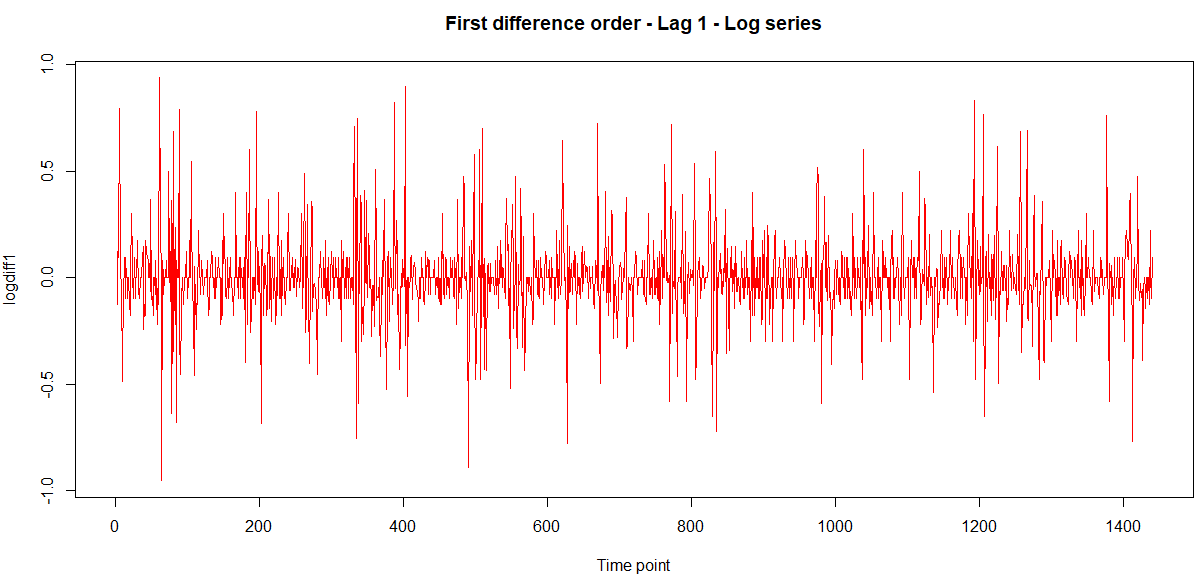
\includegraphics[width=\linewidth]{figure6.png}
  \caption{The difference series}
  \label{fig:figure6}
\end{figure}

\paragraph{}
Here, the acf and pacf seems to be in good shape. The acf spikes at the first few lags (1 to 3)  and shows some autocorrelation at the first few lags, then quickly goes to zero afterwards. The pacf show signs of exponential decay and most pacf values are within the 95 confident interval. Figure ~\ref{fig:figure7}
\begin{figure}[H]
  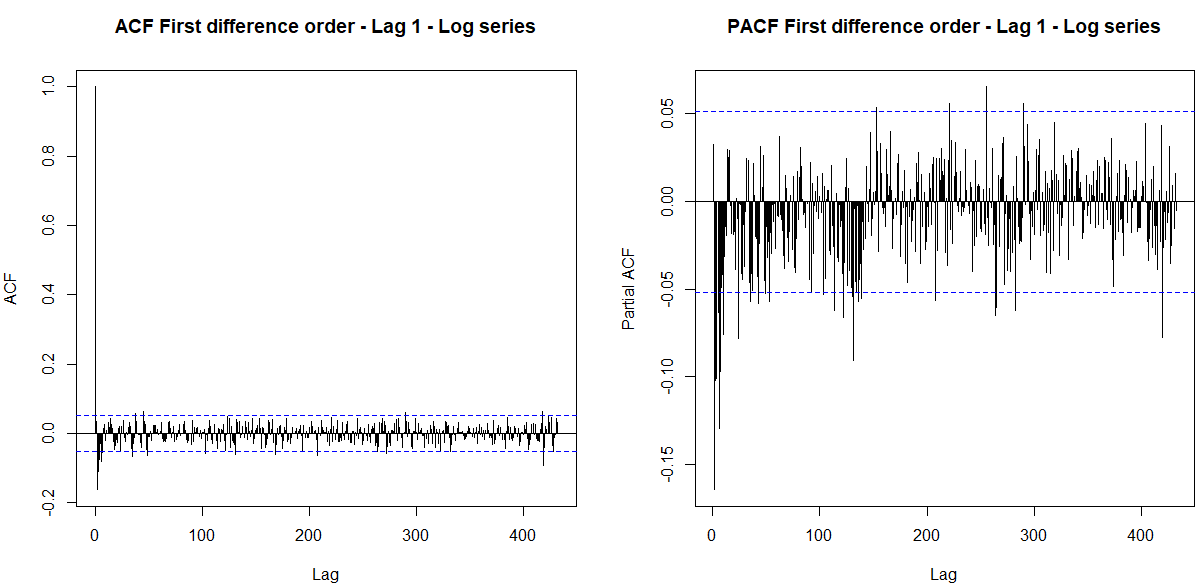
\includegraphics[width=\linewidth]{figure7.png}
  \caption{The acf and pacf plots of the difference series}
  \label{fig:figure7}
\end{figure}

\paragraph{}
To ensure stationarity, the Augmented Dickey-Fuller Test test is conducted. The null hypothesis is: 'The series is non-stationary'. The alternative hypothesis is: 'The series is stationary. Figure~\ref{fig:figure8}  shows that the p value is small enough (under 0.05) to reject the null hypothesis, accepting the alternative hypothesis. 
\begin{figure}[H]
  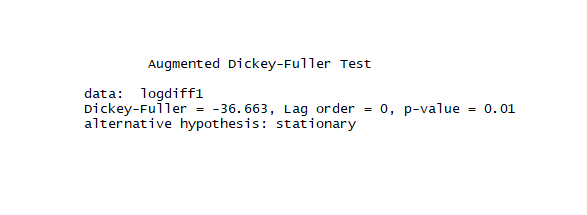
\includegraphics[width=\linewidth]{figure8.png}
  \caption{The p-value is smaller than the 0.05 $\alpha$-level }
  \label{fig:figure8}
\end{figure}

\paragraph{}
After the first few steps of exploration, it could be concluded that analysis should be done on the difference series resulting from taking the first order difference of the log series at lag 1. Because the variance is now more stable and the  series is stationary in mean, therefore, is more suitable for model fitting than the original series.
 
\section{Models}
\paragraph{}
The general approach for applying models is: 
\begin{itemize}
  \item Fitting the models on a sample of 10 days 
  \item Evaluating the goodness of fit of the models
  \item Evaluating the accuracy of the models using a test set of 12 data points ahead
\end{itemize}
\paragraph{}
Below is the list of models which will be applied:
\begin{enumerate}
  \item AR(1)
  \item AR(3)
  \item MA(1)
  \item MA(3)
  \item ARMA(3,3)
  \item ARIMA(1,1,1)(1,0,1)[144]
  \item Exponential Smoothing ($\alpha=0.9999339$)
  \item Holt's linear ($\alpha=1,\beta=0.01253426$)
  \item Holt Winter ($\alpha=0.8,\beta=0,\gamma=1$)
  \item Garch(1,1)-ARMA(1,1)
\end{enumerate}

\paragraph{}
The choice for parameters will be explained in detailed later on. The models will be presented in three groups: models that require stationary, forecasting algorithms and models that can deal with changing variance over time.
\subsection{Models that require stationary}
\paragraph{}
Refer to Figure ~\ref{fig:figure7}the acf spikes at lag 1 to 3 and the pacf has an exponential decay shape like. This indicates that an MA(3) model could be a good fit for the first order difference series of the log sample at lag 1. However, other models such as AR(1), AR(3), MA(3) are also fitted. The reason for choosing lag 3 results from observing the acf and pacf, heuristics that energy consumption levels within 30 minutes are correlated and also for the sake of reducing computational cost, AR(144) could not be fitted. Figure~\ref{fig:figure9}  and Figure ~\ref{fig:figure10}  show how the fitting looks like among the four models after undifferencing.
\begin{figure}[H]
  \centering
  \begin{subfigure}[b]{0.9\linewidth}
    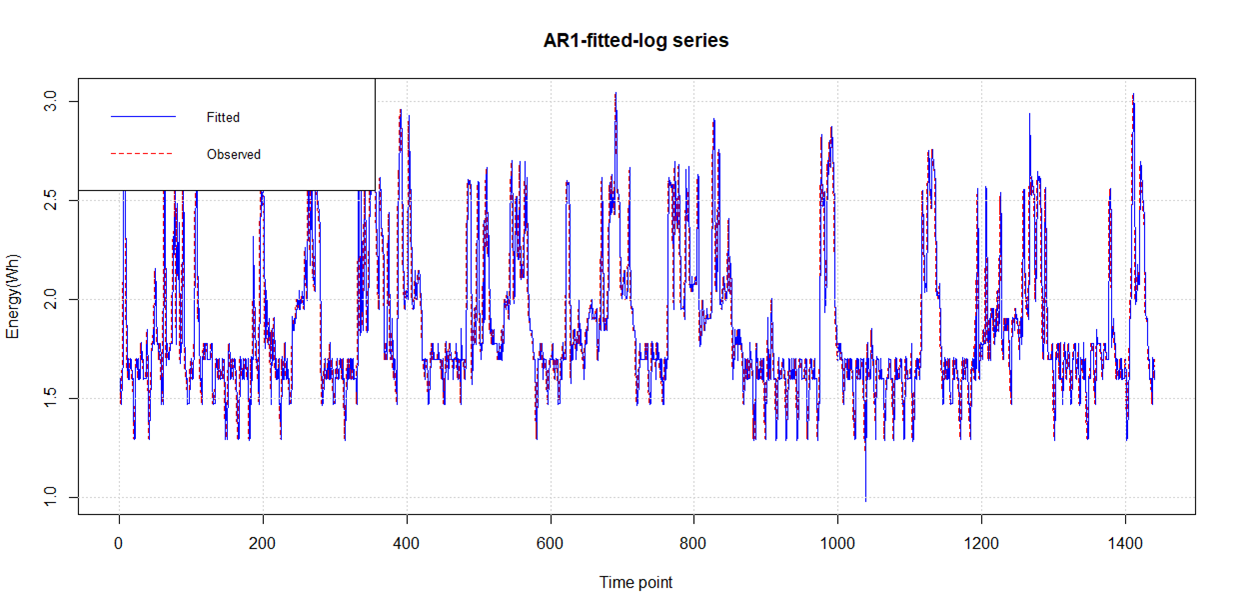
\includegraphics[width=\linewidth]{figure9-1.png}
  \end{subfigure}
  \begin{subfigure}[b]{0.9\linewidth}
    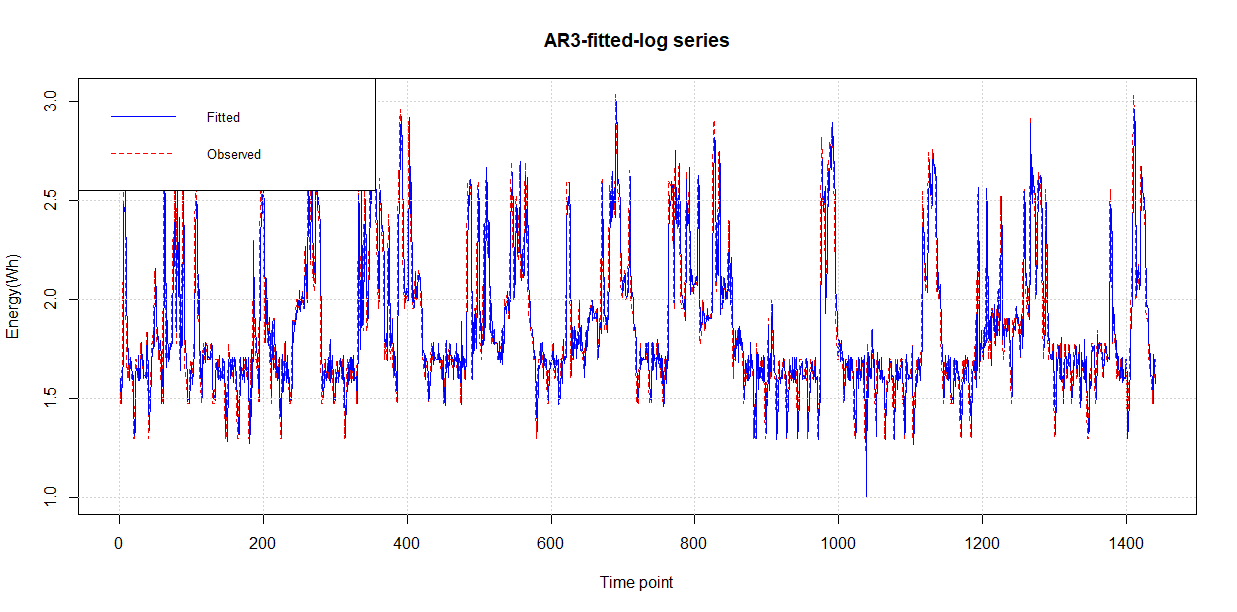
\includegraphics[width=\linewidth]{figure9-2.png}
  \end{subfigure}
  \caption{AR models}
  \label{fig:figure9}
\end{figure}

\begin{figure}[H]
  \centering
  \begin{subfigure}[b]{0.9\linewidth}
    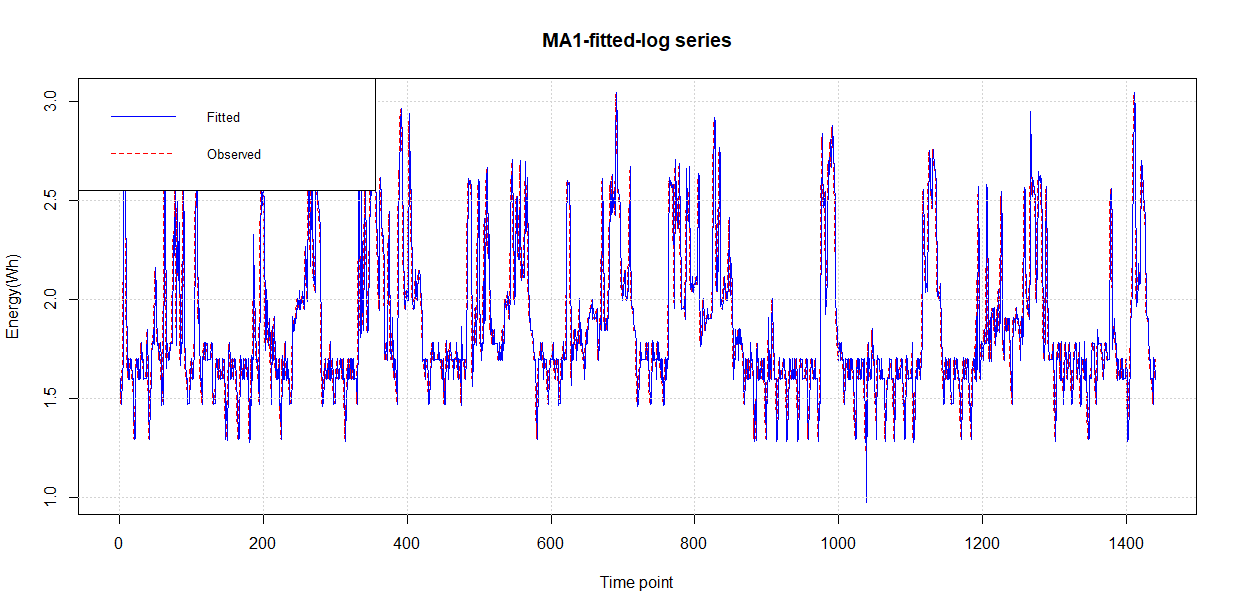
\includegraphics[width=\linewidth]{figure9-3.png}
  \end{subfigure}
  \begin{subfigure}[b]{0.9\linewidth}
    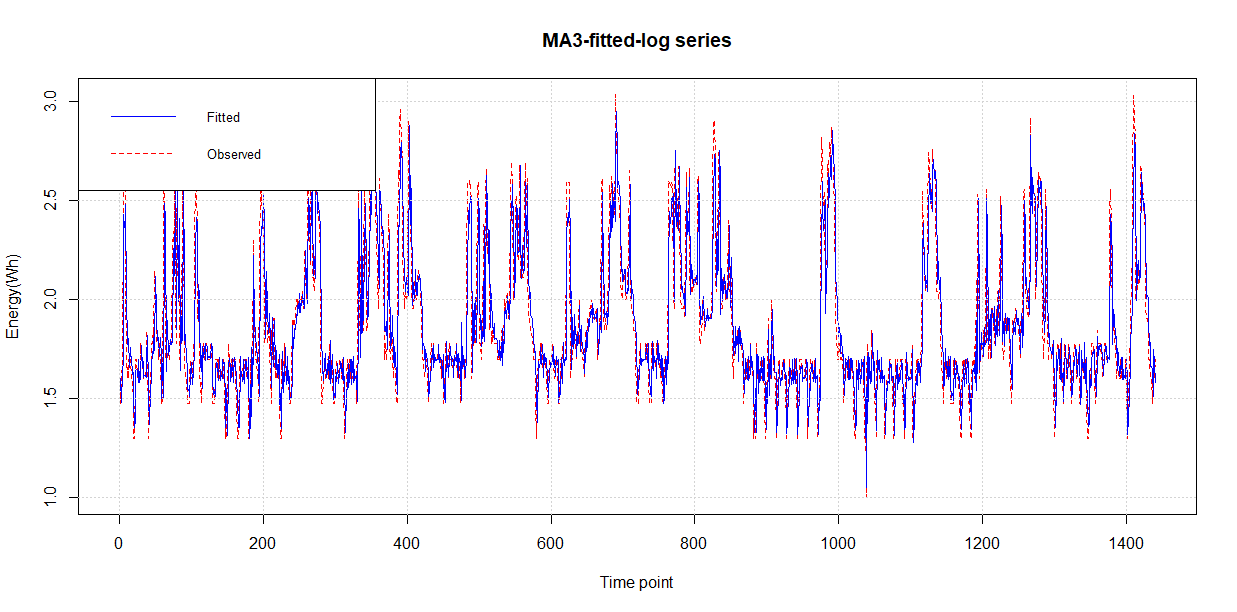
\includegraphics[width=\linewidth]{figure9-4.png}
  \end{subfigure}
  \caption{MA models}
  \label{fig:figure10}
\end{figure}

\paragraph{}
As can be seen, the fitting lines seem to be similar. It is hard to tell which model has better goodness of fit. The residual histograms, the QQ plots and the residual acf plots will then be compared. 
\begin{figure}[H]
  \centering
  \begin{subfigure}[b]{0.6\linewidth}
    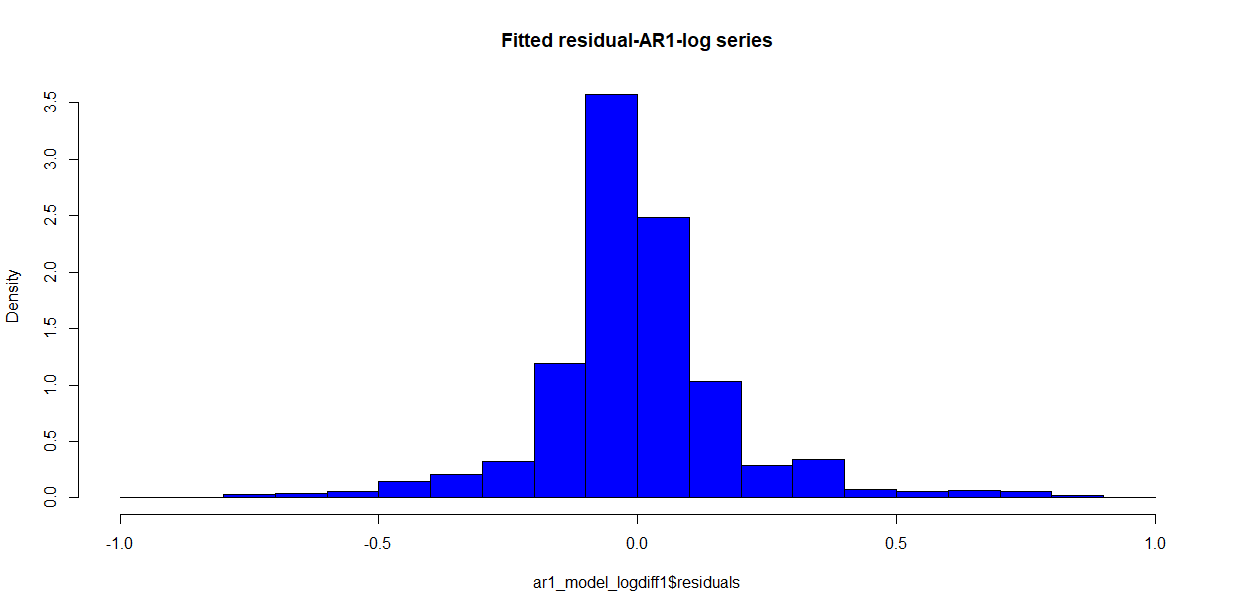
\includegraphics[width=\linewidth]{figure11-1.png}
  \end{subfigure}
  \begin{subfigure}[b]{0.6\linewidth}
    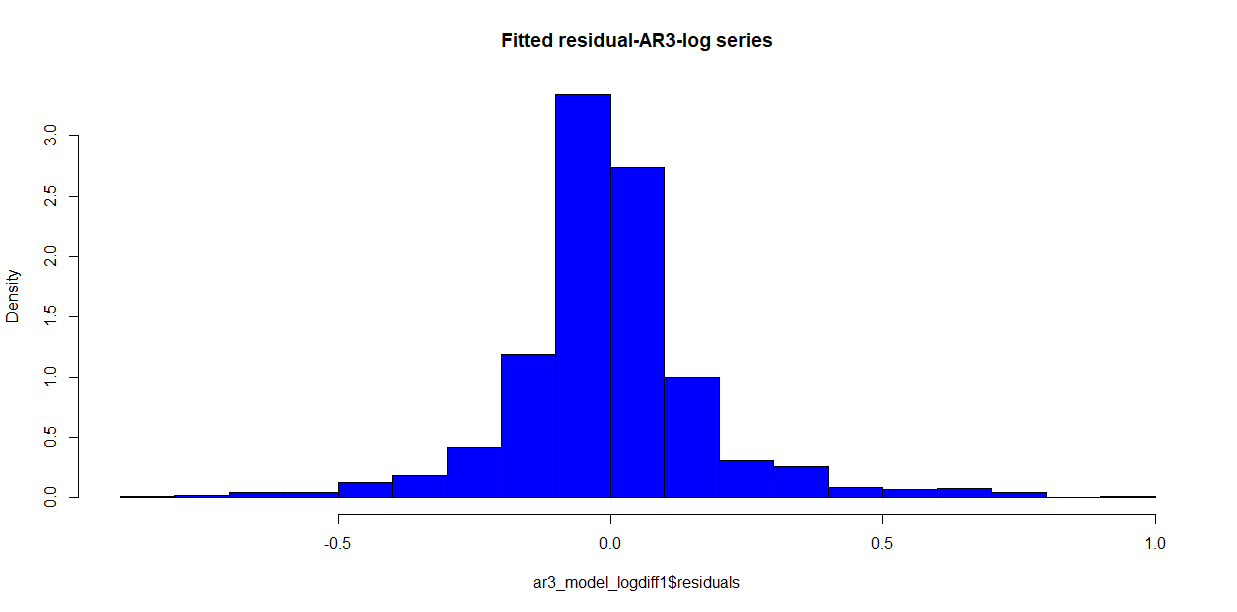
\includegraphics[width=\linewidth]{figure11-2.png}
  \end{subfigure}
  \begin{subfigure}[b]{0.6\linewidth}
    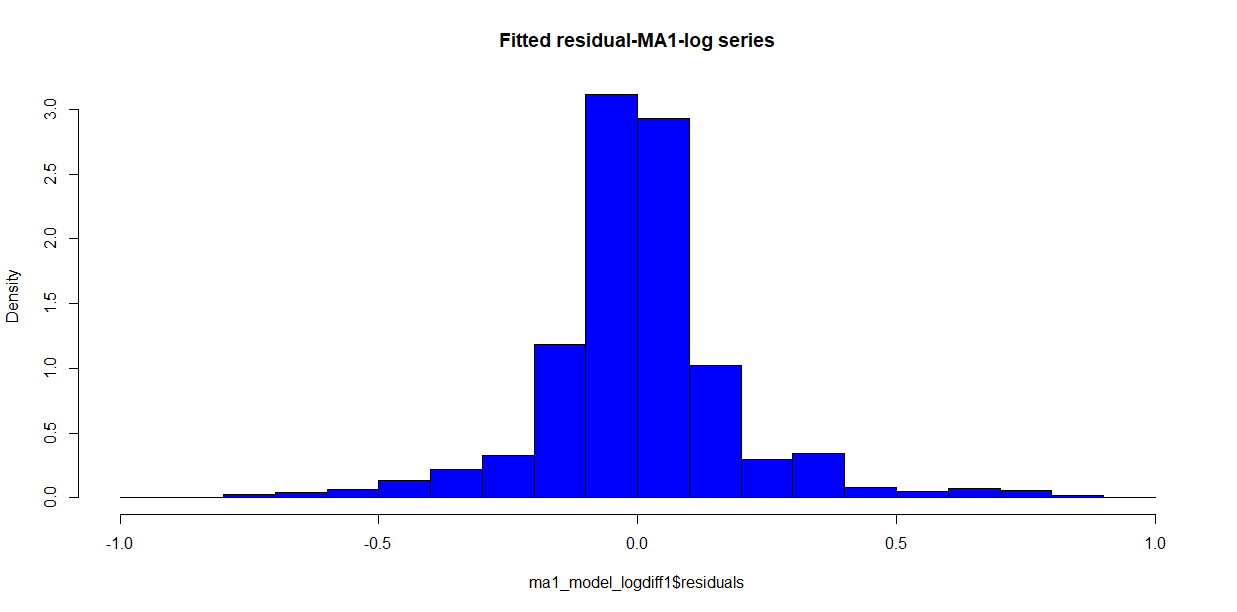
\includegraphics[width=\linewidth]{figure11-3.png}
  \end{subfigure}
  \begin{subfigure}[b]{0.6\linewidth}
    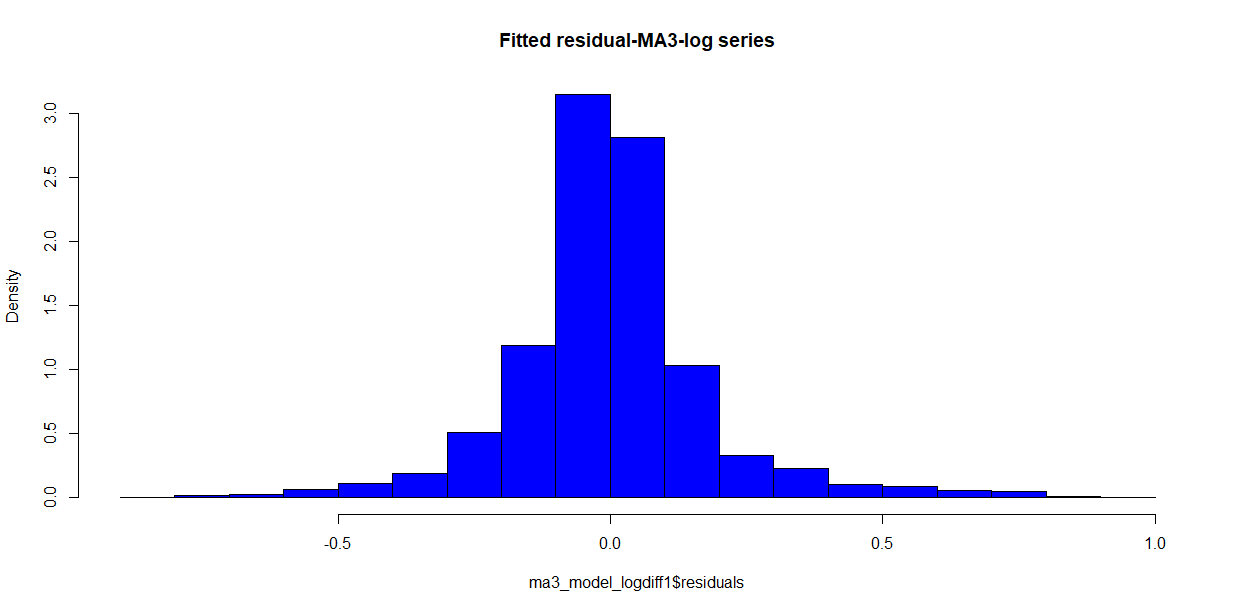
\includegraphics[width=\linewidth]{figure11-4.png}
  \end{subfigure}
  \caption{Residual histograms}
  \label{fig:figure11}
\end{figure}
\paragraph{}
As can be seen, the histograms from the MA models are a bit more symmetrical and normal than those of the AR models. This could be due to the characteristics described in Figure ~\ref{fig:figure7}. Next QQ plots are observed.
\begin{figure}[H]
  \centering
  \begin{subfigure}[b]{0.6\linewidth}
    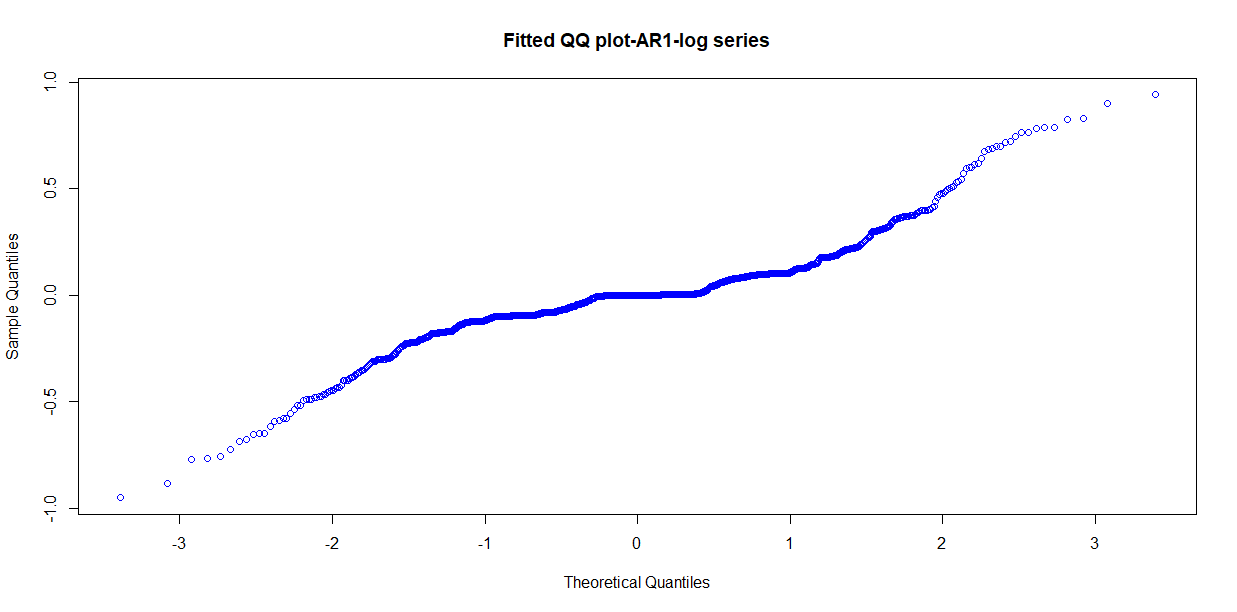
\includegraphics[width=\linewidth]{figure12-1.png}
  \end{subfigure}
  \begin{subfigure}[b]{0.6\linewidth}
    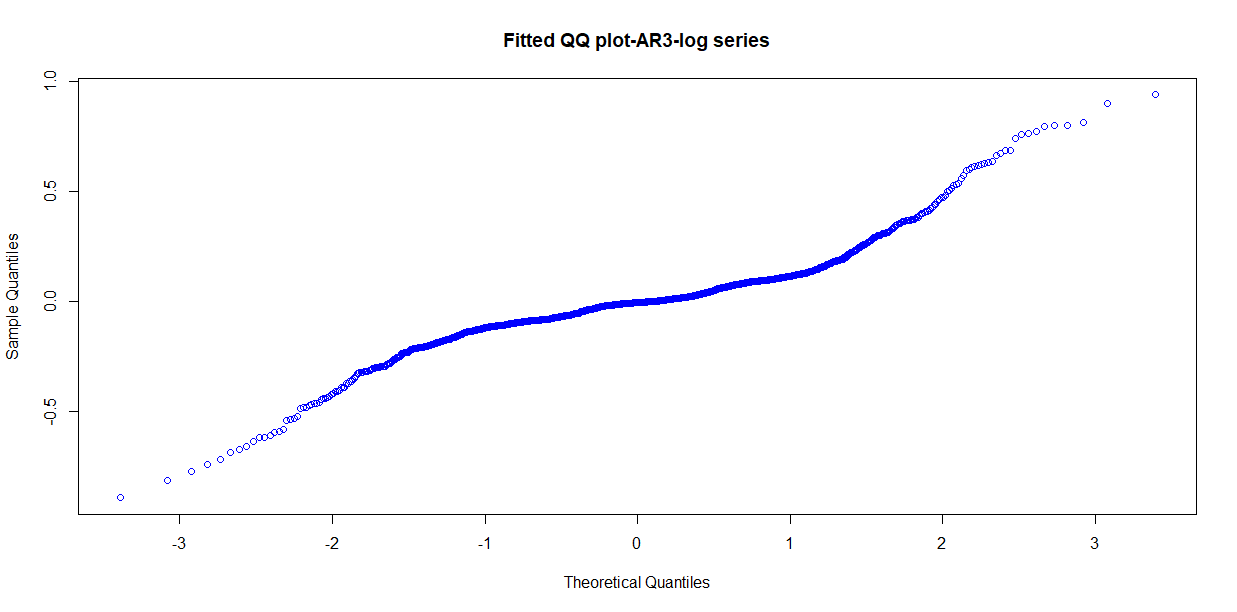
\includegraphics[width=\linewidth]{figure12-2.png}
  \end{subfigure}
  \begin{subfigure}[b]{0.6\linewidth}
    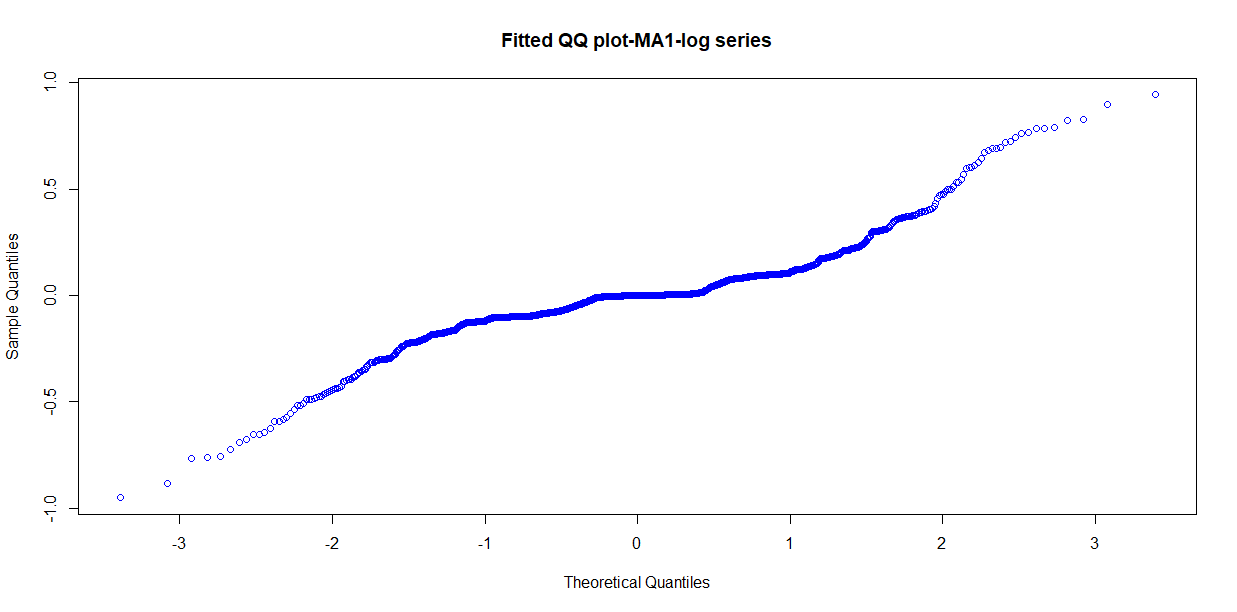
\includegraphics[width=\linewidth]{figure12-3.png}
  \end{subfigure}
  \begin{subfigure}[b]{0.6\linewidth}
    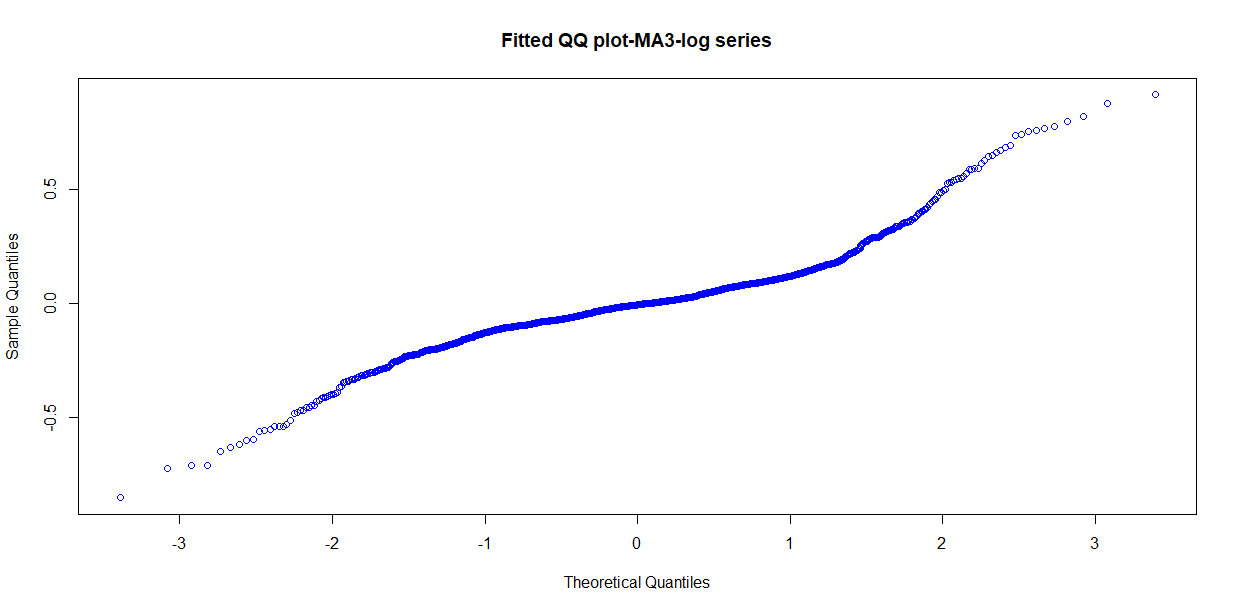
\includegraphics[width=\linewidth]{figure12-4.png}
  \end{subfigure}
  \caption{QQ plots}
  \label{fig:figure12}
\end{figure}
\paragraph{}
Overall, MA models also have better QQ plots. MA(3) seems to have the points form the 'straightest' line. To compare further goodness of fit, MAPE and AIC of the models are computed. These two measures are chosen since MAPE does not depends on the range of outcome values, which could be different from samples to samples, and AIC penalize the models for being overfitting. The following tables show the results of the four models.

\begin{table}[H]
  \begin{center}
    \caption{MAPE and AIC}
    \label{tab:table1}
    \begin{tabular}{c|c|S} % <-- Alignments, all center
      \textbf{Model} & \textbf{MAPE} & \textbf{AIC}\\
      \hline
      AR(1) & 0.06328462 & -664.2\\
      AR(3) & 0.06480294 & -714.86\\
      MA(1) & 0.06356587 & -664.92\\
      MA(3) & 0.06569768 & -747.59\\
    \end{tabular}
  \end{center}
\end{table}

\paragraph{}
As can be seen, the models receive similar MAPE values. However, MA(3) gets the lowest AIC values, indicating it could be best to use MA(3) in comparison with the other three models. Next, forecasts are made for the models and the MAPE values are also computed given a test set of 12 data points on the log scale. Figure ~\ref{fig:figure13}  shows the forecast of the models on the log scale. Figure ~\ref{fig:figure14}  shows the forecast of the models on the original scale.
\begin{figure}[H]
  \centering
  \begin{subfigure}[b]{0.6\linewidth}
    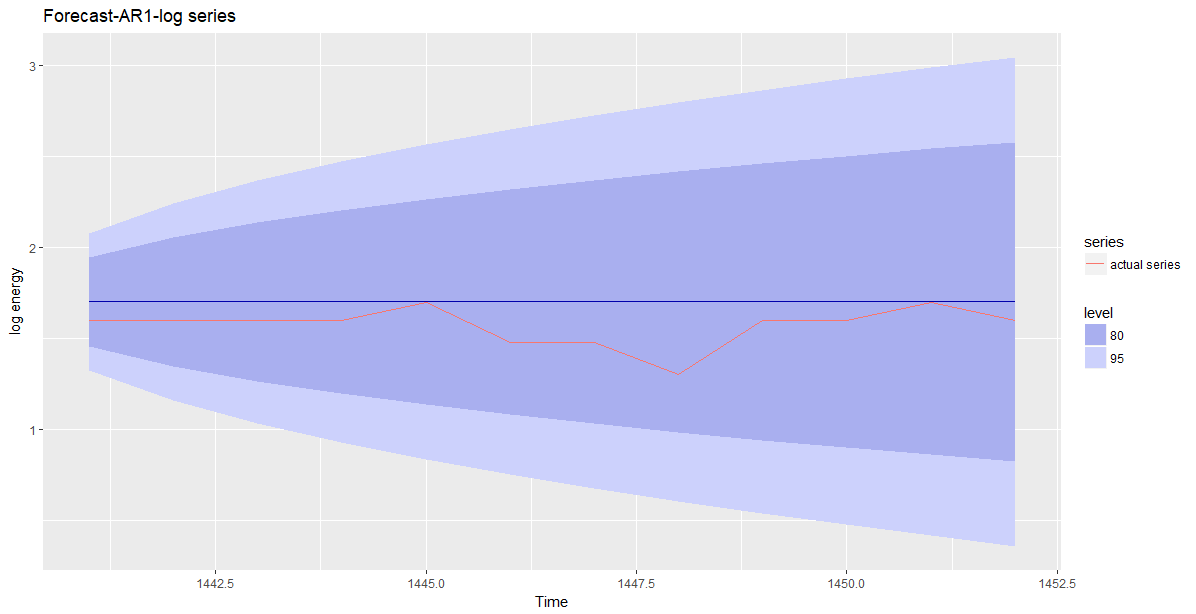
\includegraphics[width=\linewidth]{figure13-1.png}
  \end{subfigure}
  \begin{subfigure}[b]{0.6\linewidth}
    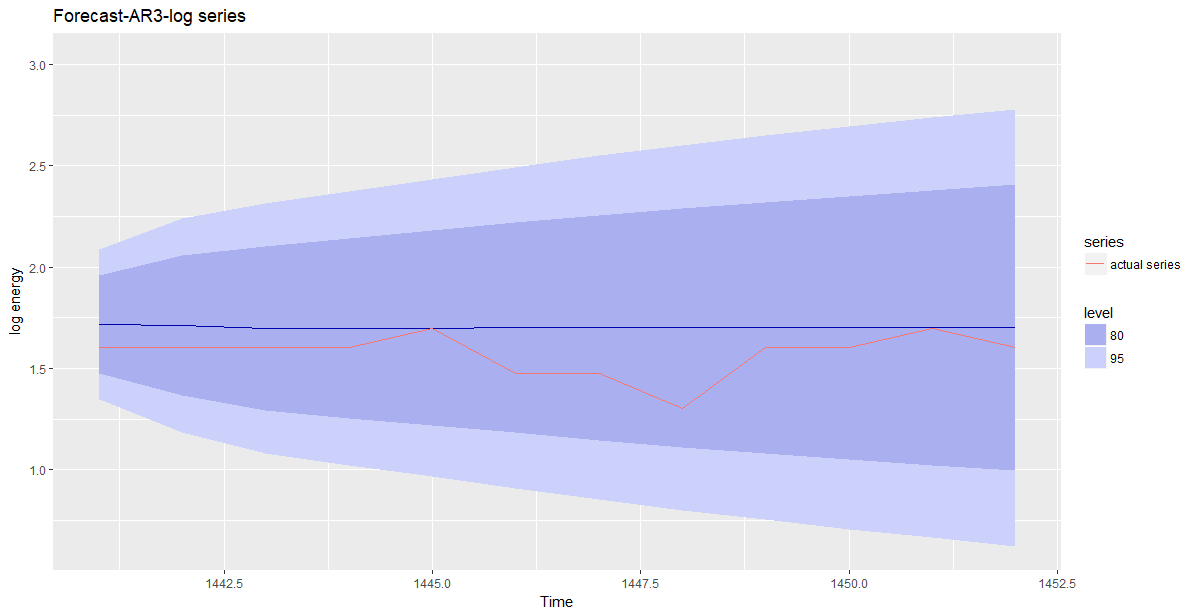
\includegraphics[width=\linewidth]{figure13-2.png}
  \end{subfigure}
  \begin{subfigure}[b]{0.6\linewidth}
    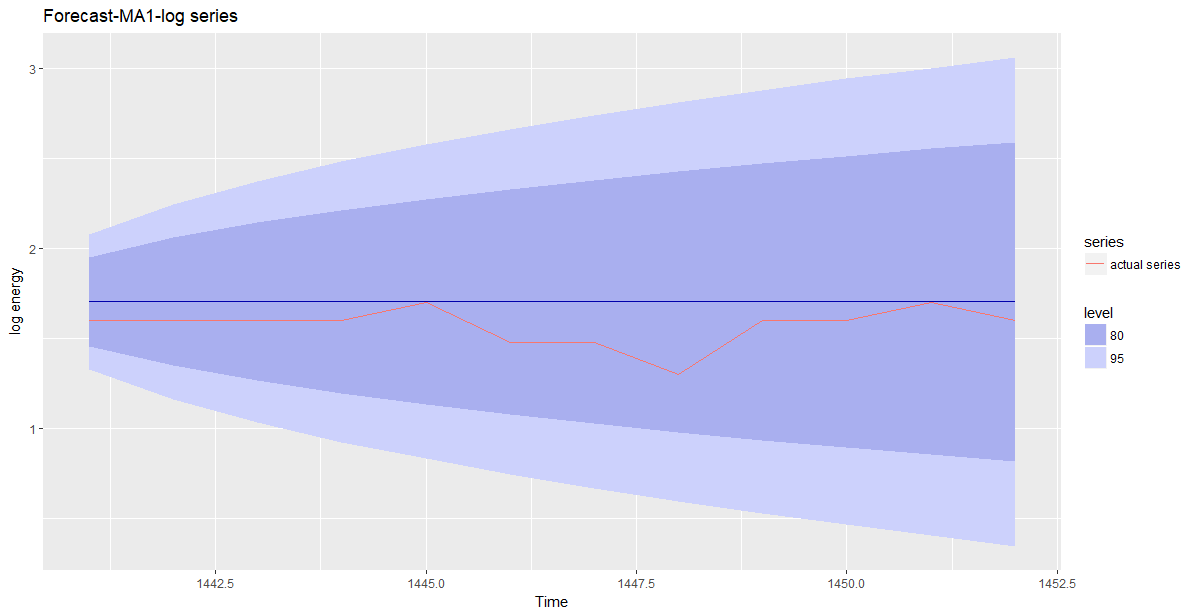
\includegraphics[width=\linewidth]{figure13-3.png}
  \end{subfigure}
  \begin{subfigure}[b]{0.6\linewidth}
    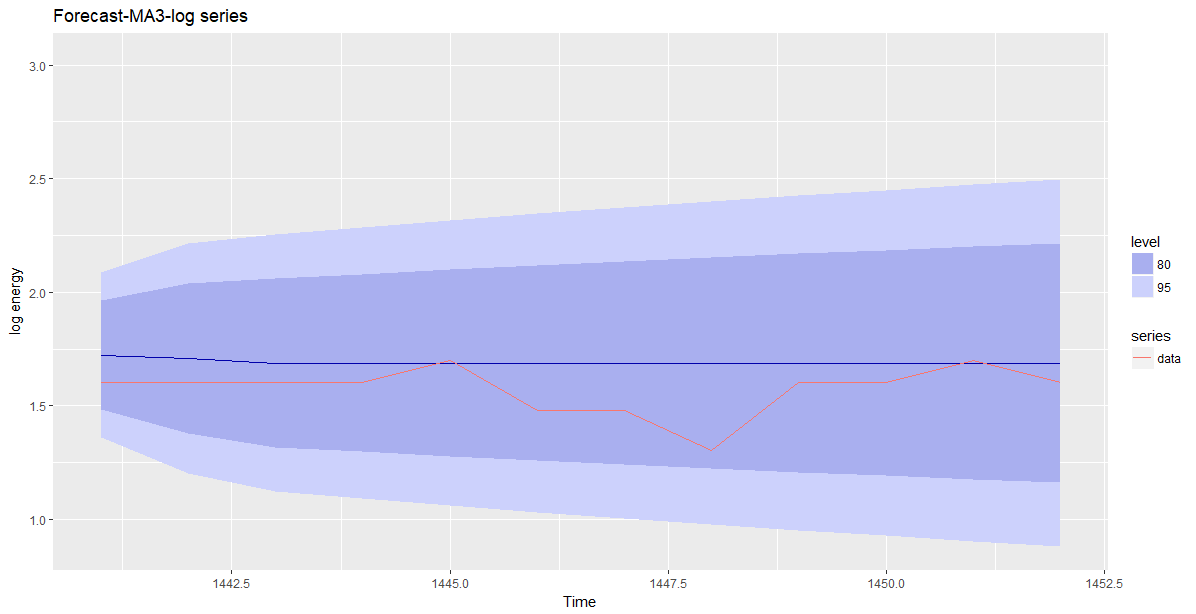
\includegraphics[width=\linewidth]{figure13-4.png}
  \end{subfigure}
  \caption{Forecast on log scale}
  \label{fig:figure13}
\end{figure}

\begin{figure}[H]
  \centering
  \begin{subfigure}[b]{0.6\linewidth}
    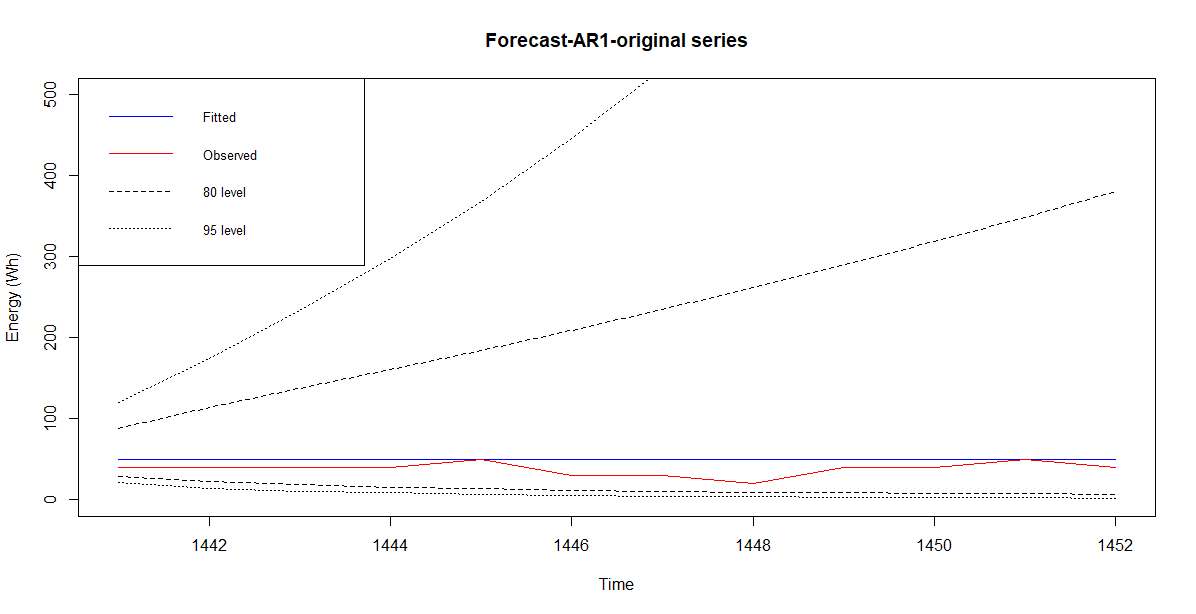
\includegraphics[width=\linewidth]{figure14-1.png}
  \end{subfigure}
  \begin{subfigure}[b]{0.6\linewidth}
    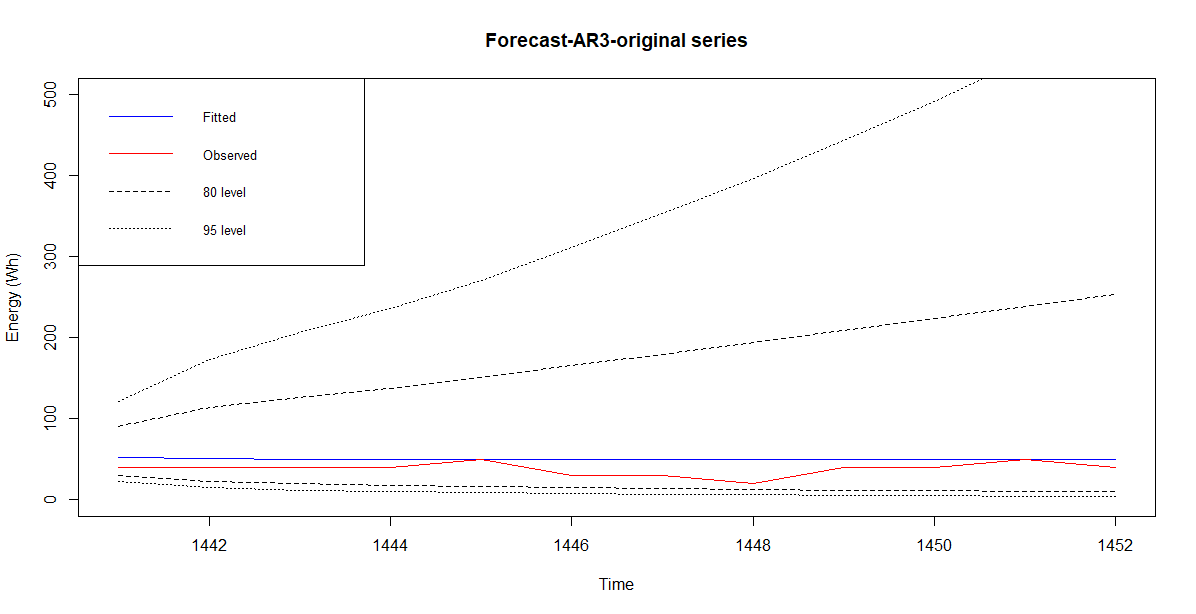
\includegraphics[width=\linewidth]{figure14-2.png}
  \end{subfigure}
  \begin{subfigure}[b]{0.6\linewidth}
    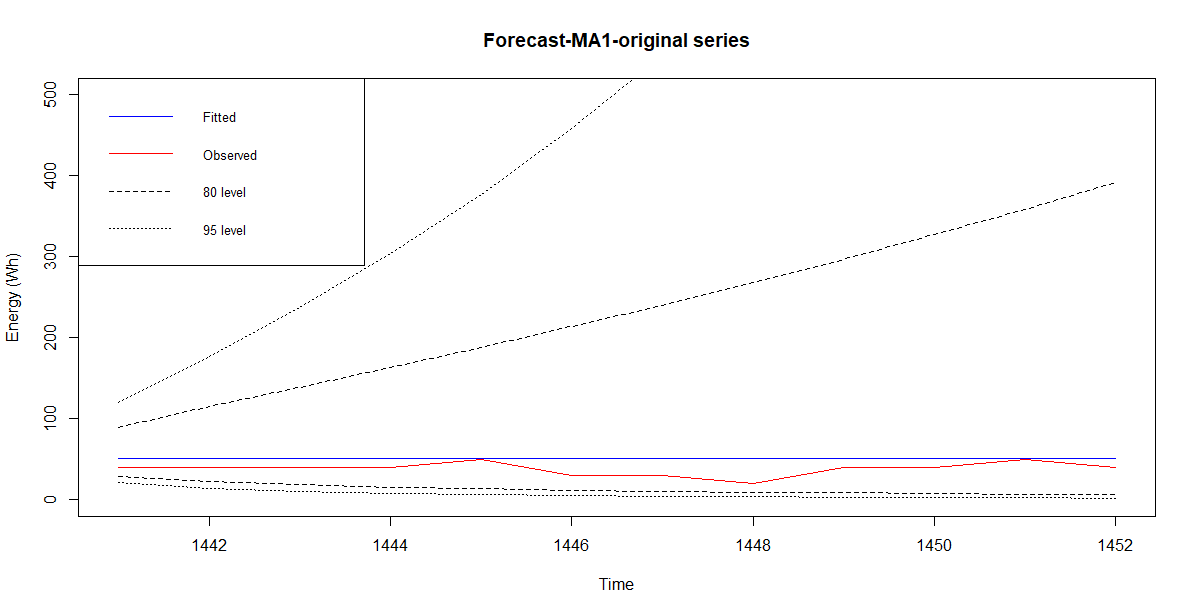
\includegraphics[width=\linewidth]{figure14-3.png}
  \end{subfigure}
  \begin{subfigure}[b]{0.6\linewidth}
    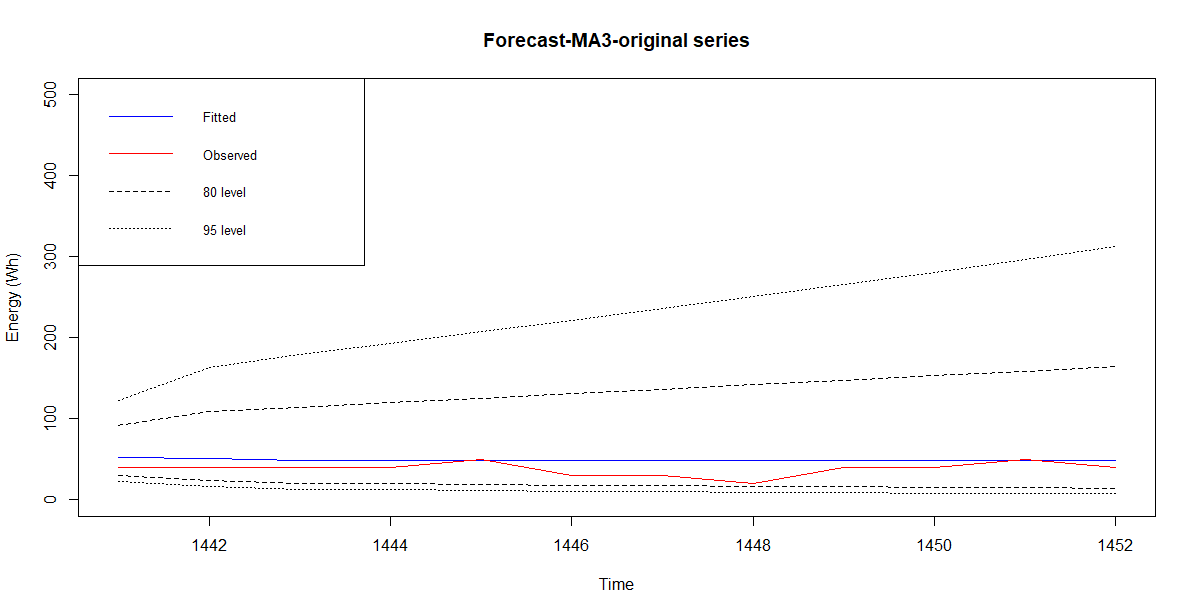
\includegraphics[width=\linewidth]{figure14-4.png}
  \end{subfigure}
  \caption{Forecast on orginal scale}
  \label{fig:figure14}
\end{figure}

\paragraph{}
On both scales, MA(3) shows to have the smallest 95 confident interval. All the models give similar predictions. Table ~\ref{tab:table2} shows the MAPE computed on the given test set on the log scale. Again, MA(3) has the lowest test MAPE among the models. Other models receive similar test MAPE values. 
\begin{table}[H]
  \begin{center}
    \caption{Test MAPE}
    \label{tab:table2}
    \begin{tabular}{c|c|S} % <-- Alignments, all center
      \textbf{Model} & \textbf{MAPE}\\
      \hline
      AR(1) & 0.08789718\\
      AR(3) & 0.08798882\\
      MA(1) & 0.08889993\\
      MA(3) & 0.08400015\\
    \end{tabular}
  \end{center}
\end{table}

\paragraph{}
In order to attempt decreasing the test MAPE and the AIC, ARIMA with a seasonal components is applied. For model specification, these values are set: $(p,d,q)=(1,0,1), (P,D,Q)=(1,1,1)$ and $s=144$. This model is applied on the log series. The seasonal length is 144 because there are 144 10-minute intervals within a day. First, the log series is differenced by 1 season at first order, then 1 seasonal lag is applied to the series in both AR and MA parts. Next, the normal ARMA(1,1) process is applied. Figure ~\ref{fig:figure15} shows the process of fitting the model.
\begin{figure}[H]
  \centering
  \begin{subfigure}[b]{0.6\linewidth}
    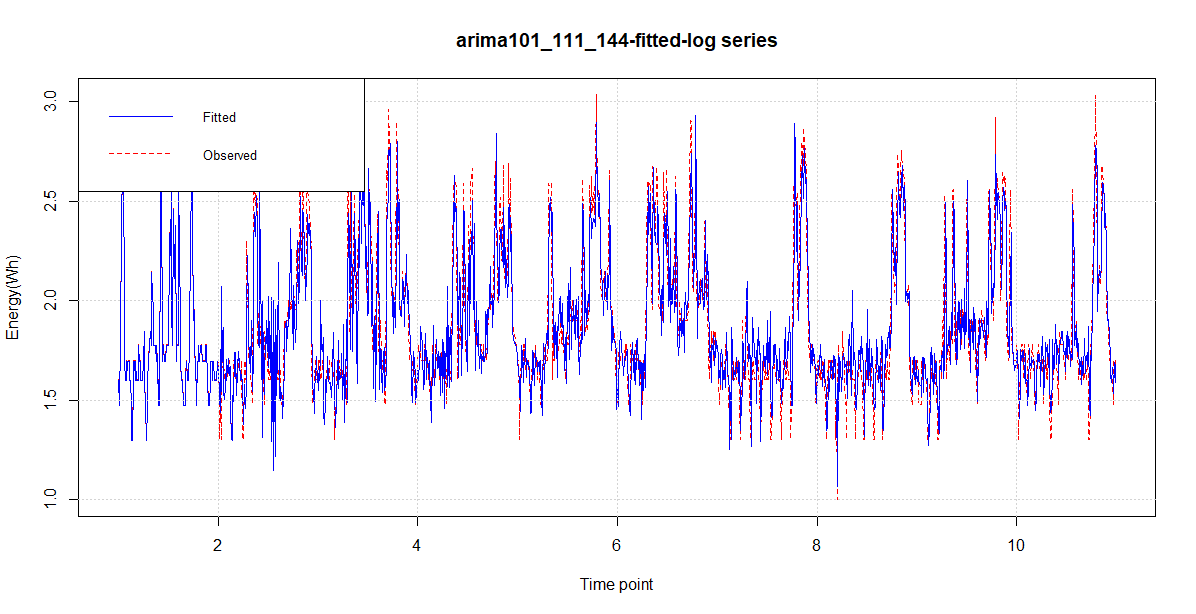
\includegraphics[width=\linewidth]{figure15-1.png}
  \end{subfigure}
  \begin{subfigure}[b]{0.6\linewidth}
    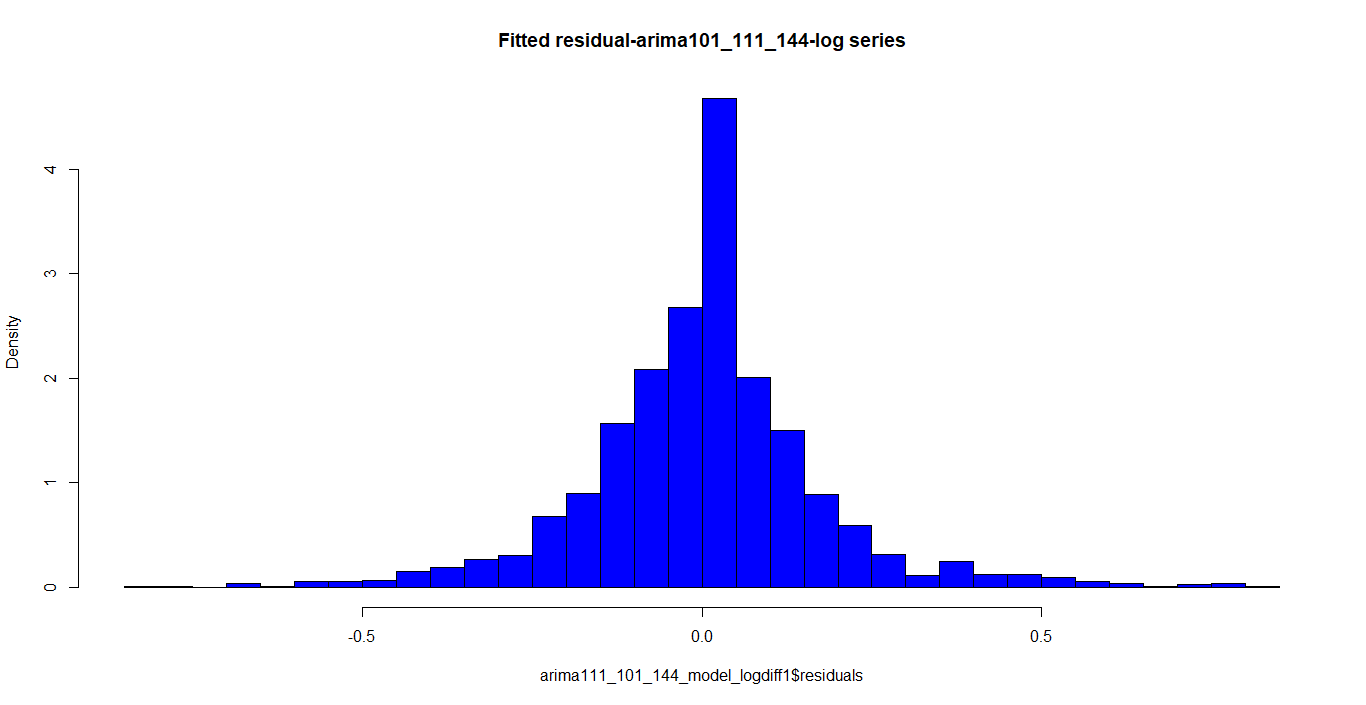
\includegraphics[width=\linewidth]{figure15-2.png}
  \end{subfigure}
  \begin{subfigure}[b]{0.6\linewidth}
    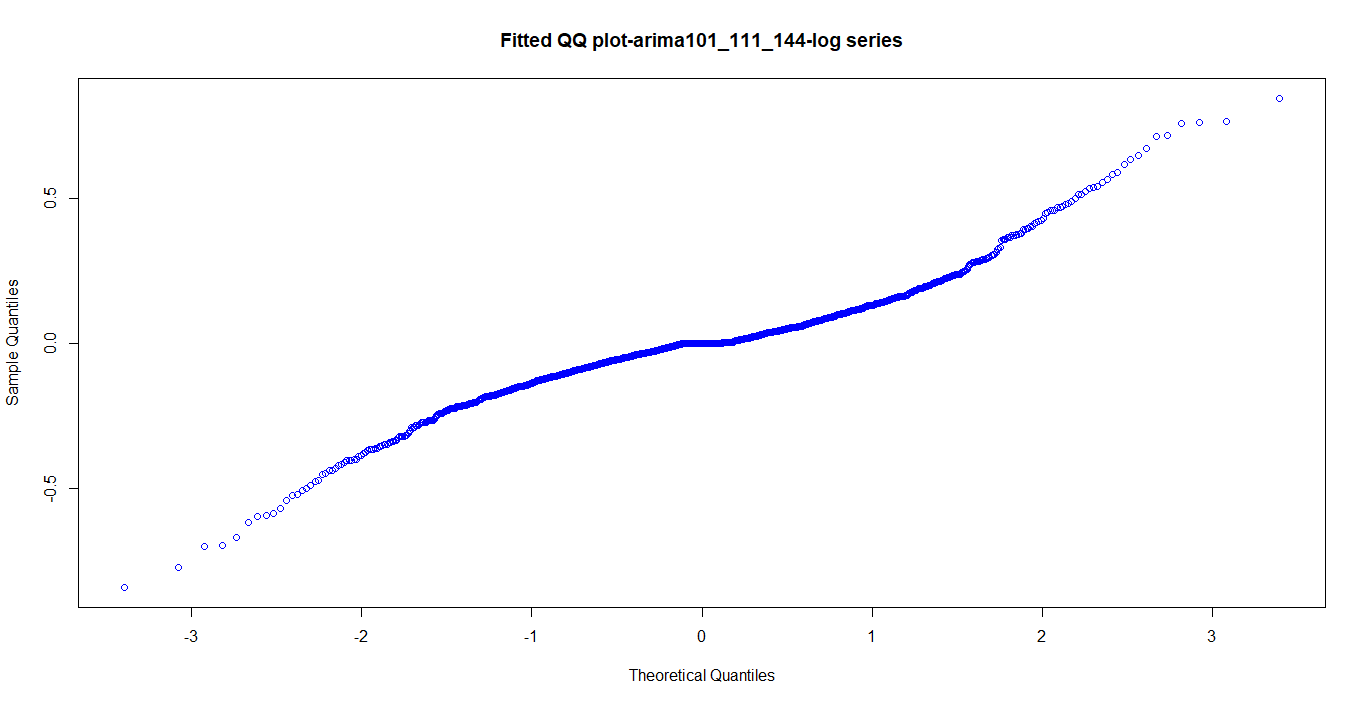
\includegraphics[width=\linewidth]{figure15-3.png}
  \end{subfigure}
  \begin{subfigure}[b]{0.6\linewidth}
    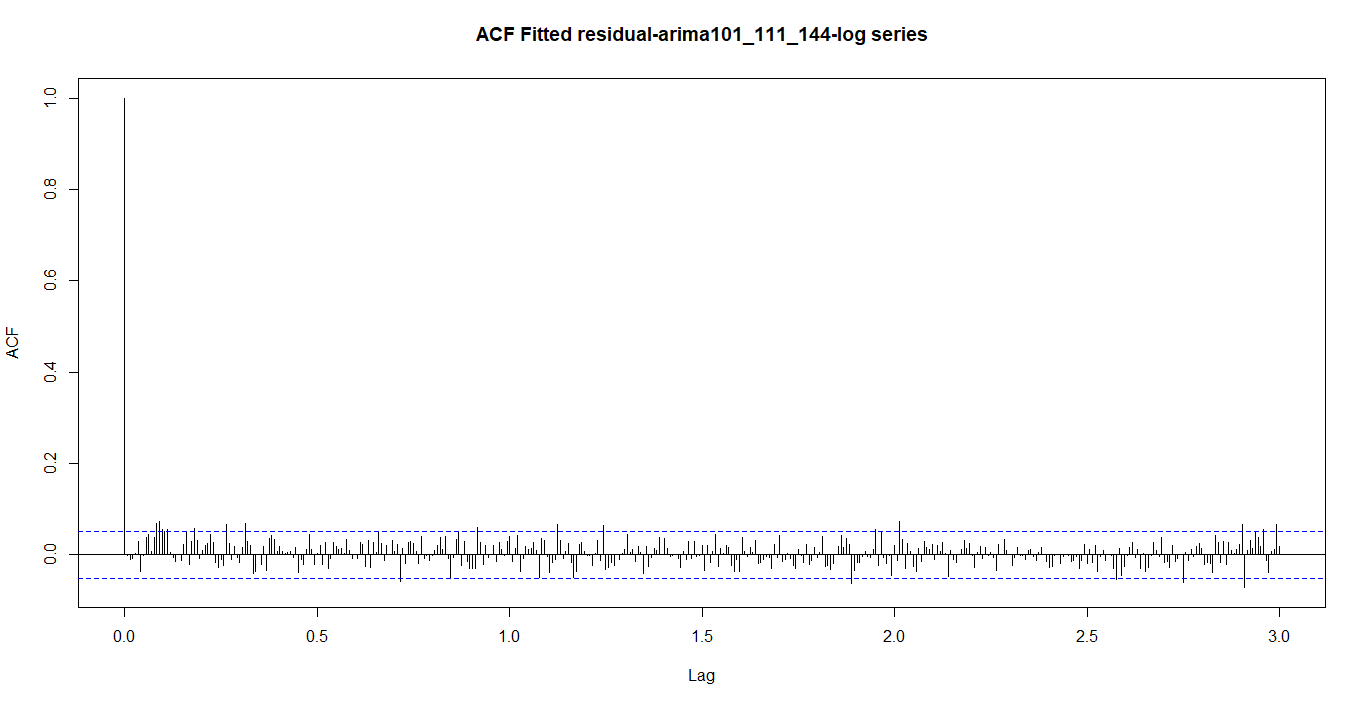
\includegraphics[width=\linewidth]{figure15-4.png}
  \end{subfigure}
  \caption{ARIMA(1,0,1)(1,1,1)[144]. Fitted plot - Residual histogram - QQ plot - ACF of residuals}
  \label{fig:figure15}
\end{figure}

\paragraph{}
Both the histogram and the QQ plot are in quite nice normal shape. The acf also shows low autocorrelation in the residuals. For this model, the fitting MAPE is 0.0636094, which is quite low compared to previous models. However, the AIC of this model sees a higher value of -458.34 (refer back to table ~\ref{tab:table1} for comparison). This could be showing that the model is more overfitting compared to the others. In fact, the test MAPE of this model is 0.09180982, which is also higher than previous models (refer back to table ~\ref{tab:table2} comparison). This observation indicates that this complex model is more overfitting. The forecasts in the log scale and the original scale is shown in Figure ~\ref{fig:figure16}.
\begin{figure}[H]
  \centering
  \begin{subfigure}[b]{1\linewidth}
    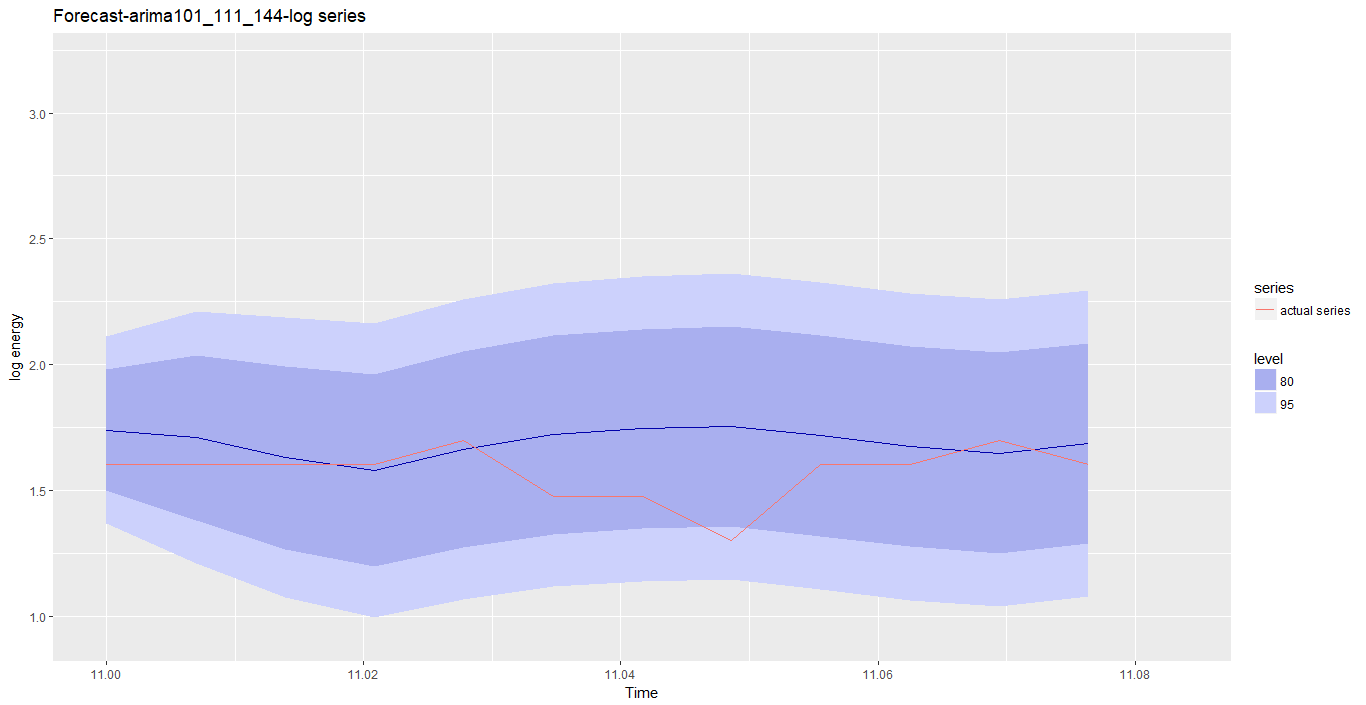
\includegraphics[width=\linewidth]{figure15-5.png}
  \end{subfigure}
  \begin{subfigure}[b]{1\linewidth}
    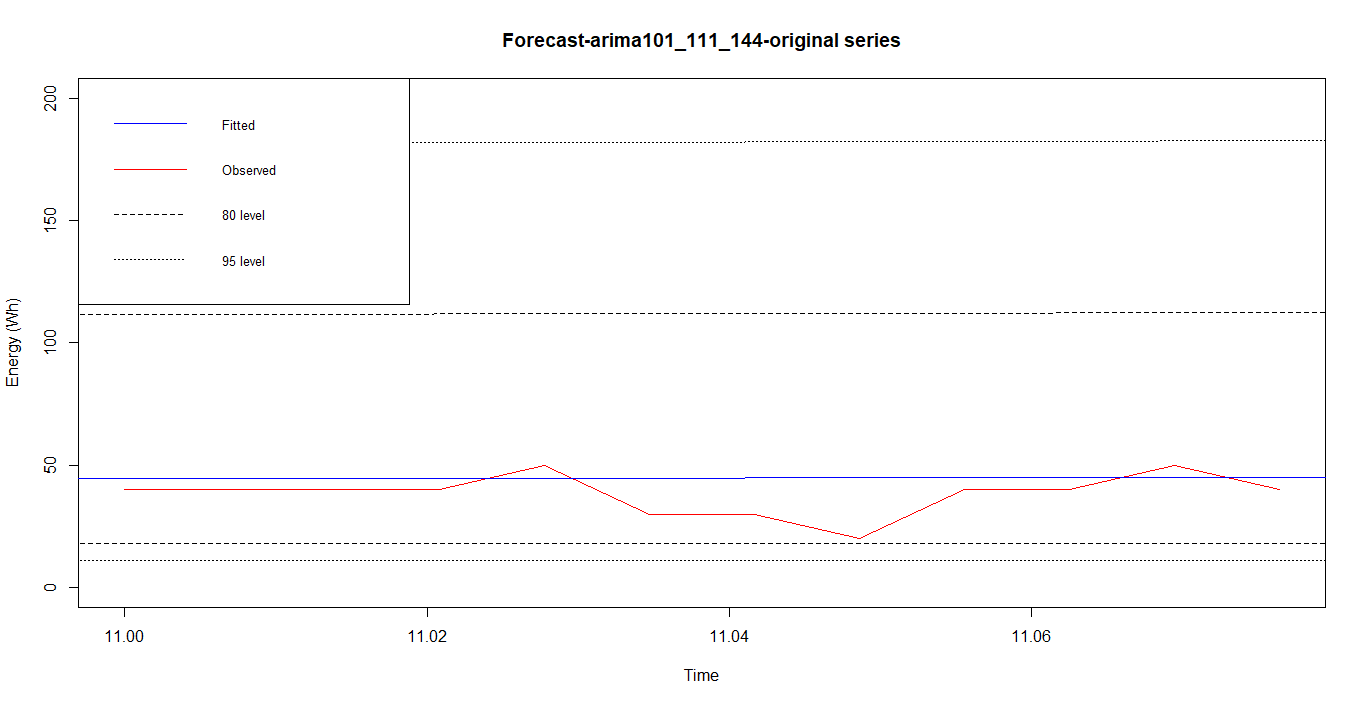
\includegraphics[width=\linewidth]{figure15-6.png}
  \end{subfigure}
  \caption{ARIMA(1,0,1)(1,1,1)[144] - forecast}
  \label{fig:figure16}
\end{figure}

\paragraph{}
Next, the function auto.arima() in R is applied to seek for the optimal ARIMA model for this log series. The function returns an ARIMA(3,0,3) model, which is also an ARIMA(3,3) model. This model receives the lowest AIC so far, hitting -803.36. However, the MAPE in both the fitting and the forecasting process are not among the lowest ones. Surprisingly, the test MAPE value is quite high compared to other models (0.1371812). Figure ~\ref{fig:figure17} shows all the common process for this model.
\begin{figure}[H]
  \centering
  \begin{subfigure}[b]{0.6\linewidth}
    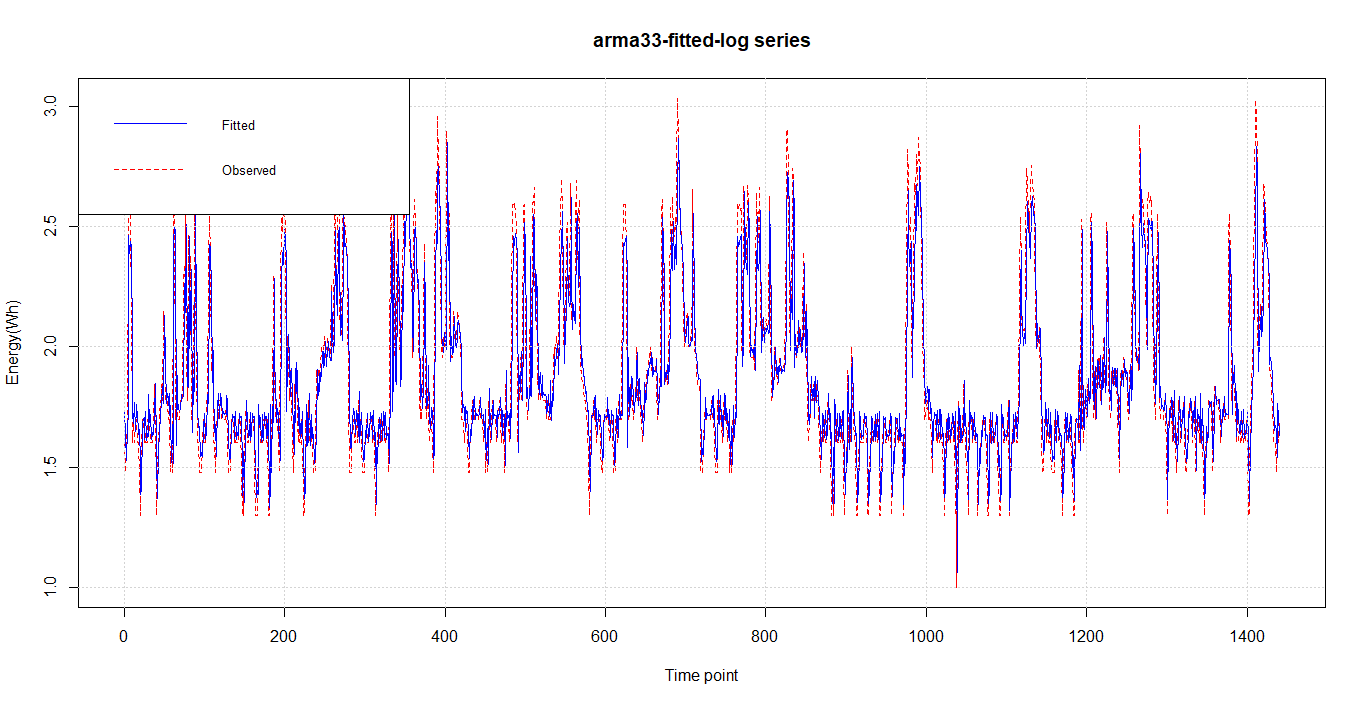
\includegraphics[width=\linewidth]{figure16-1.png}
  \end{subfigure}
  \begin{subfigure}[b]{0.6\linewidth}
    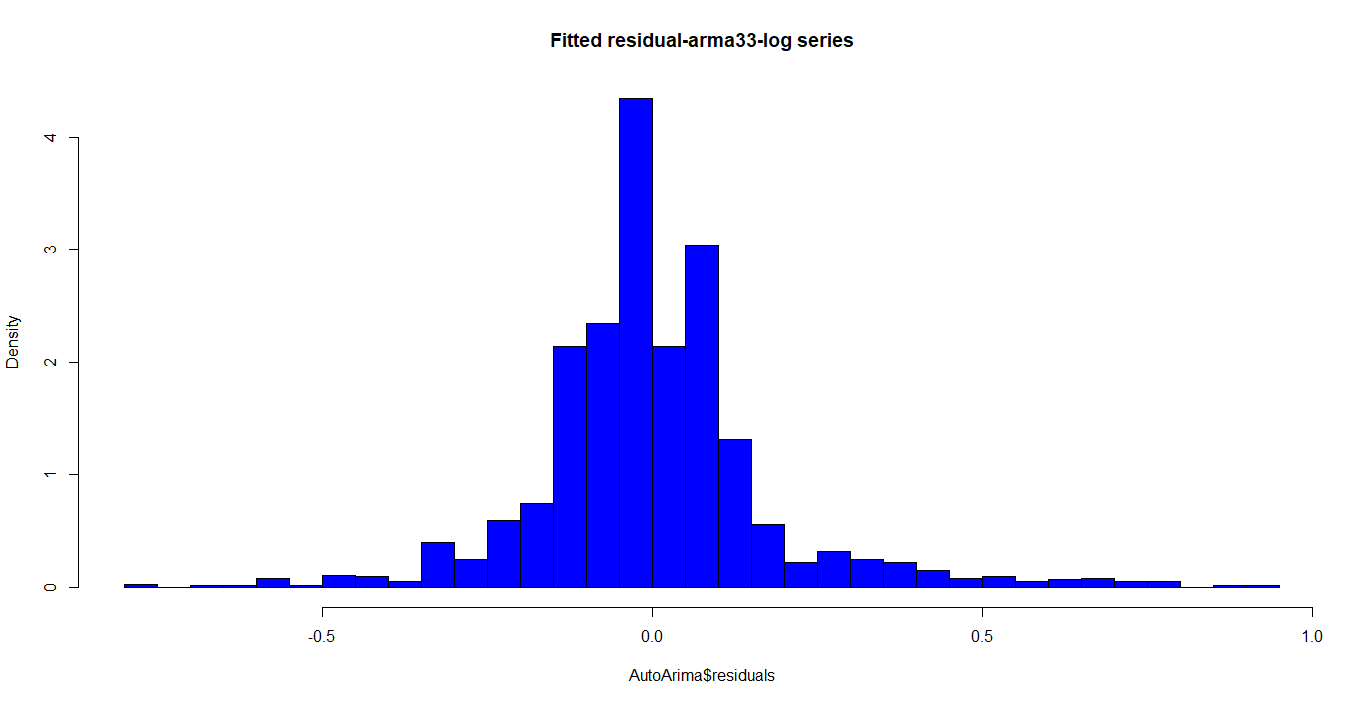
\includegraphics[width=\linewidth]{figure16-2.png}
  \end{subfigure}
  \begin{subfigure}[b]{0.6\linewidth}
    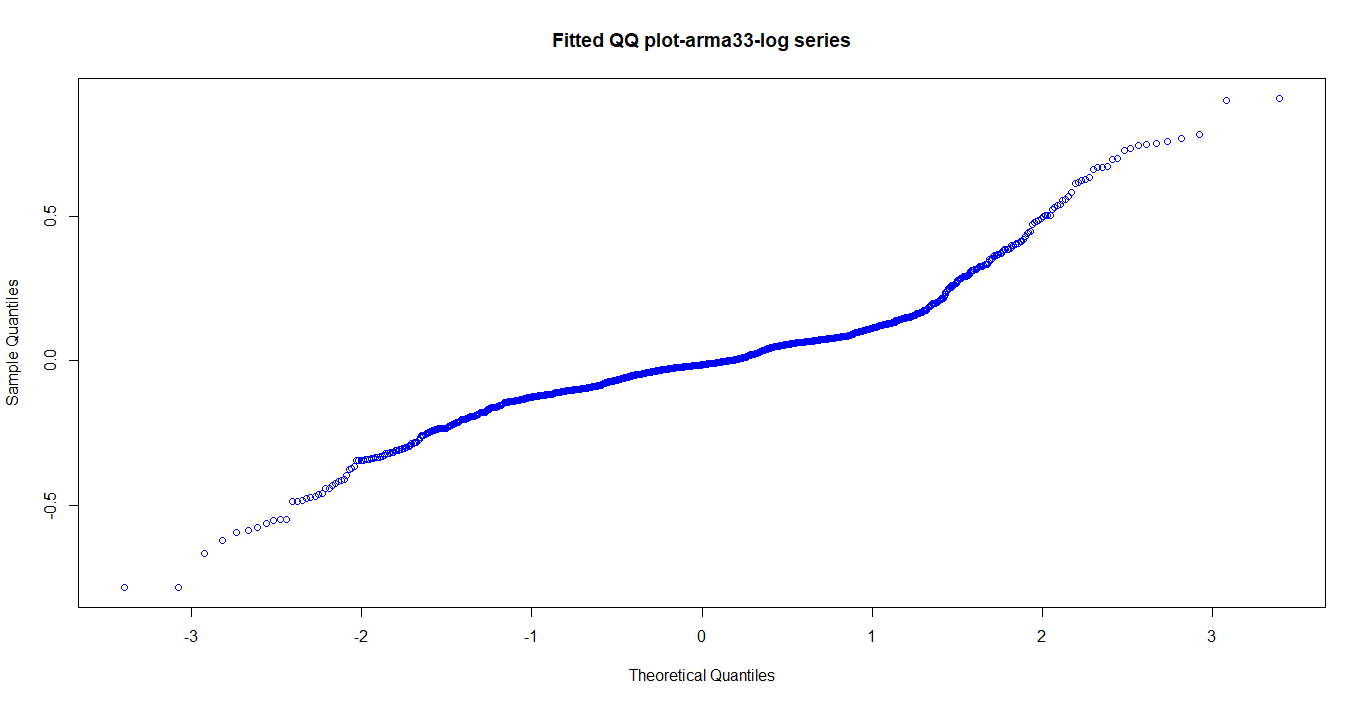
\includegraphics[width=\linewidth]{figure16-3.png}
  \end{subfigure}
  \begin{subfigure}[b]{0.6\linewidth}
    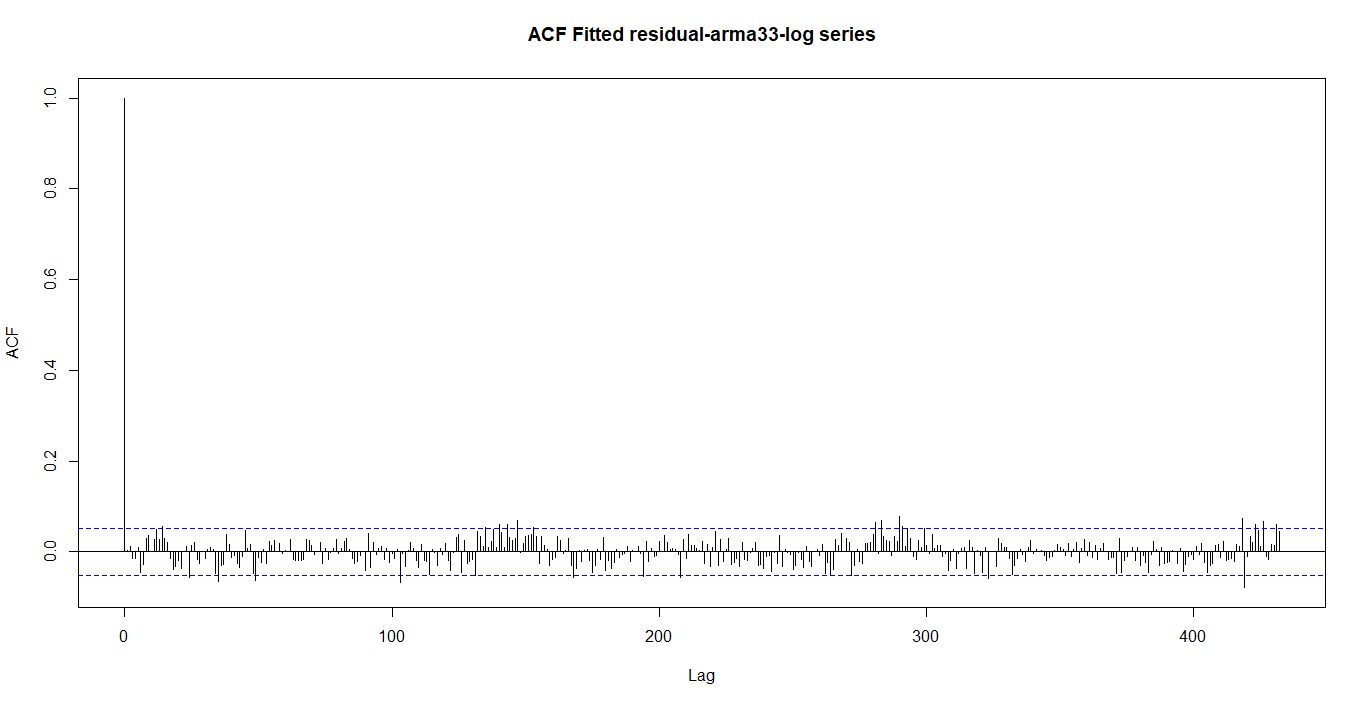
\includegraphics[width=\linewidth]{figure16-4.png}
  \end{subfigure}
  \begin{subfigure}[b]{0.6\linewidth}
    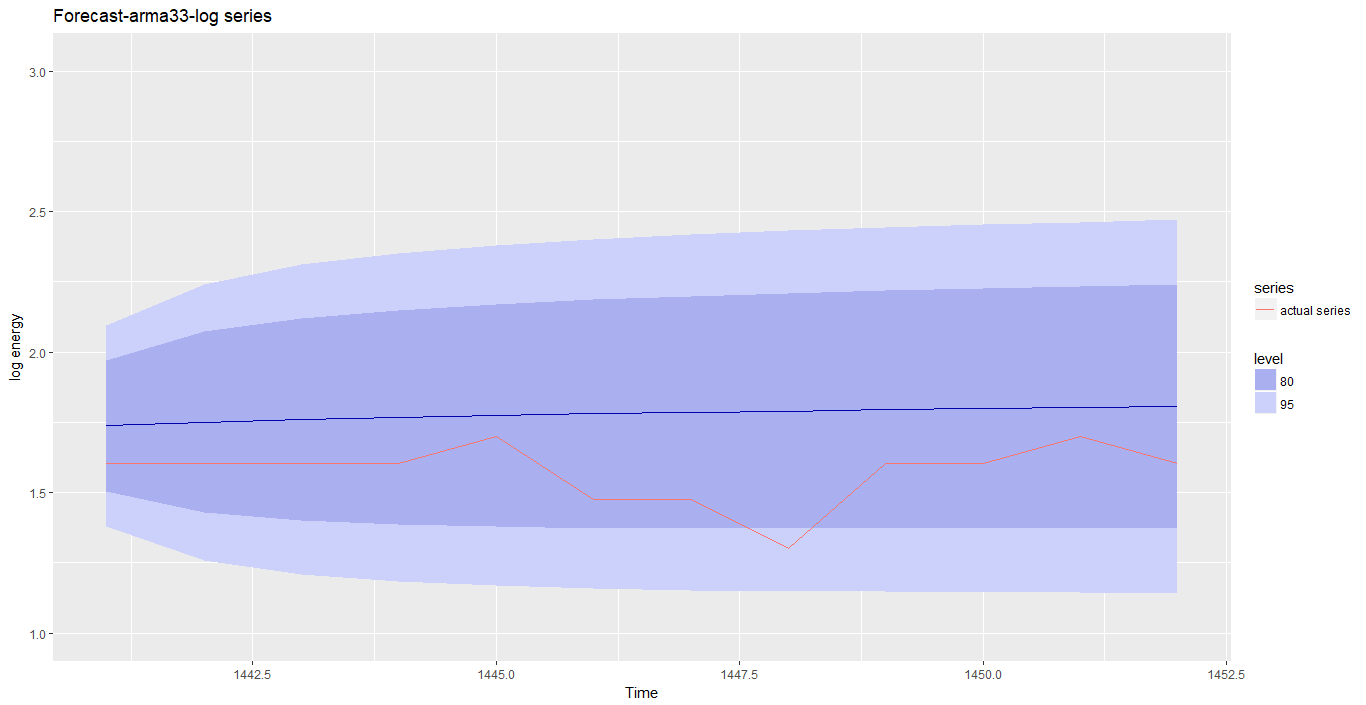
\includegraphics[width=\linewidth]{figure16-5.png}
  \end{subfigure}
  \begin{subfigure}[b]{0.6\linewidth}
    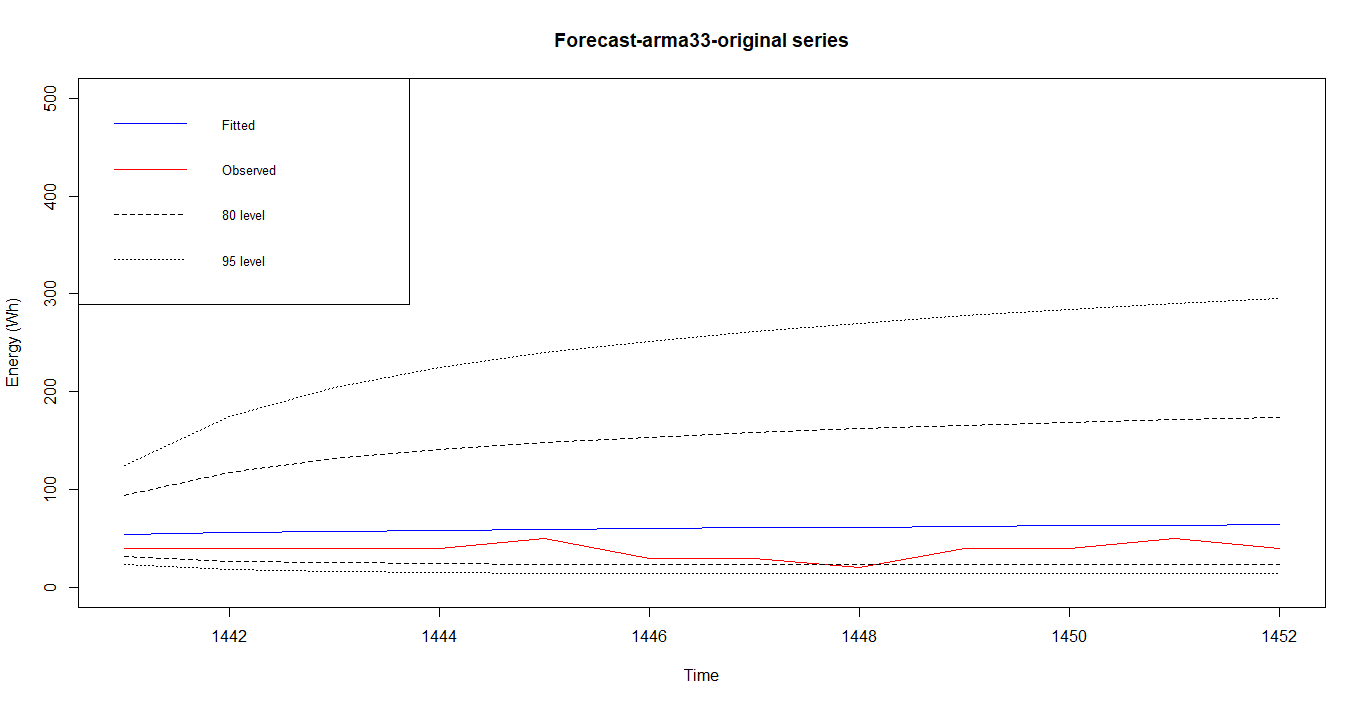
\includegraphics[width=\linewidth]{figure16-6.png}
  \end{subfigure}
  \caption{ARMA(3,3)}
  \label{fig:figure17}
\end{figure}

\paragraph{}
The histogram, QQ plot of the residuals are quite normal. However, the acf still shows some patterns and the forecasts in both the original scale and the log scale are obviously worse compared to other models. The following table summary the measures of fit for all the fitted models so far.
\begin{table}[H]
  \begin{center}
    \caption{MAPE and AIC}
    \label{tab:table3}
    \begin{tabular}{c|S|S|S} % <-- Alignments, all center
      \textbf{Model} & \textbf{MAPE} & \textbf{AIC}& \textbf{Test MAPE}\\
      \hline
      AR(1) & 0.06328462 & -664.2 & 0.08789718\\
      AR(3) & 0.06480294 & -714.86 & 0.08798882\\
      MA(1) & 0.06356587 & -664.92 & 0.08889993\\
      MA(3) & 0.06569768 & -747.59 & 0.08400015\\
      ARIMA(1,0,1)(1,1,1)[144] & 0.0636094 & -458.34 & 0.09180982\\
      ARMA(3,3) & 0.06448967 & -803.36 & 0.1371812 \\
    \end{tabular}
  \end{center}
\end{table}

\paragraph{}
From analysis on different plots, together with the results presented in Table 3, MA(3) should be chosen over the ARMA(3,3).
Although it does not have the lowest AIC, the test MAPE make up for that. Besides, its AIC value is the second lowest among the others. 

\subsection{Forecasting algorithms}
\paragraph{}
The one of the common points of these algorithms is that they contains some parameter ranging from 0 to 1. One must decide which value of each parameter for the model to work well. The proposed approach is plotting the RMSE against several values of each parameter of the algorithm to investigate the effects of each parameter on the performance of the model. These are the models to be presented in this section:
\begin{enumerate}
  \item Exponential Smoothing ($\alpha=0.9999339$)
  \item Holt's linear ($\alpha=1,\beta=0.01253426$)
  \item Holt Winter ($\alpha=0.8,\beta=0,\gamma=1$)
\end{enumerate}

\paragraph{}
First, Exponential Smoothing is attempted for the original series. This algorithm contains only one parameter. Figure ~\ref{fig:figure18} shows the effect of $\alpha$ on the RMSE of the model.
\begin{figure}[H]
  \centering
  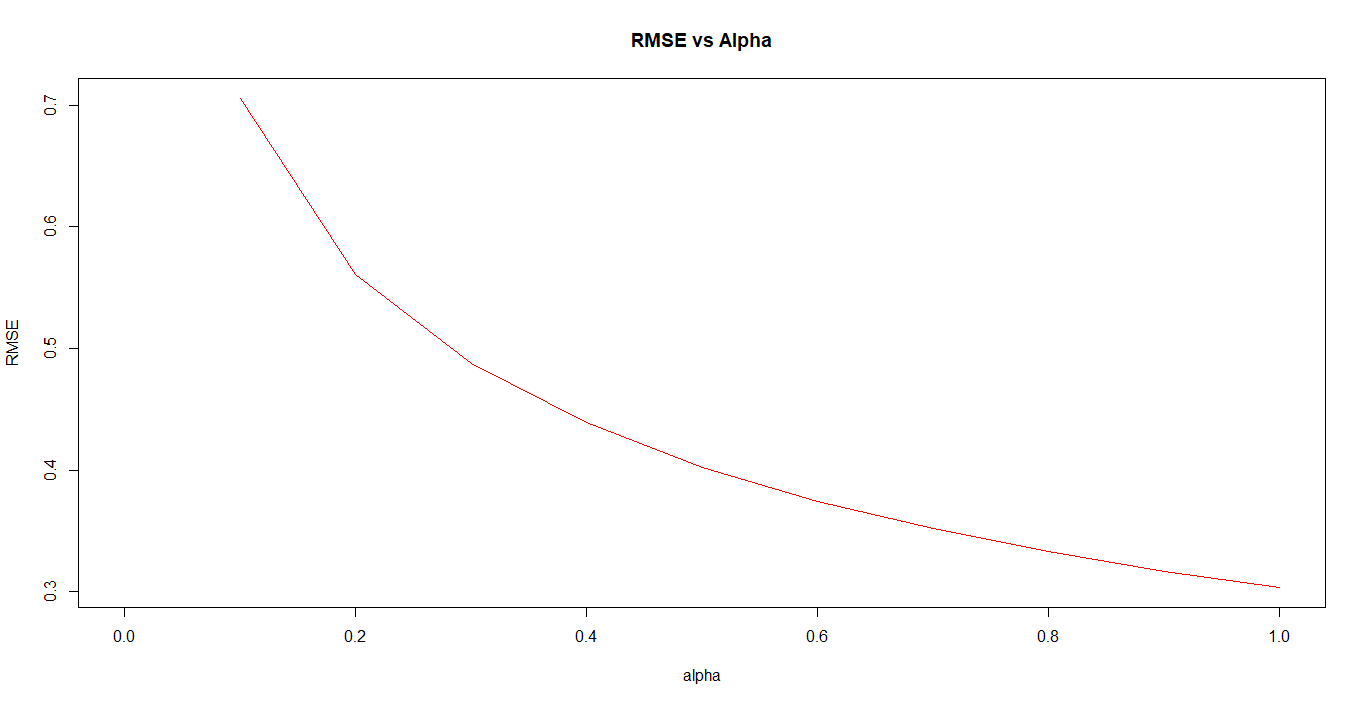
\includegraphics[width=\linewidth]{figure18.png}
  \caption{The effect of $\alpha$}
  \label{fig:figure18}
\end{figure}

\paragraph{}
As $\alpha$ increases, the RMSE tends to decrease. One can expect that the optimal value of alpha for this algorithm should be close to 1. The function HoltWinters() is used to help search for the optimal value of $\alpha$. After running, the function returns the optimal model as Exponential Smoothing ($\alpha=0.9999339$). Figure ~\ref{fig:figure19} shows the quality of fit of the model 
\begin{figure}[H]
  \centering
  \begin{subfigure}[b]{0.6\linewidth}
    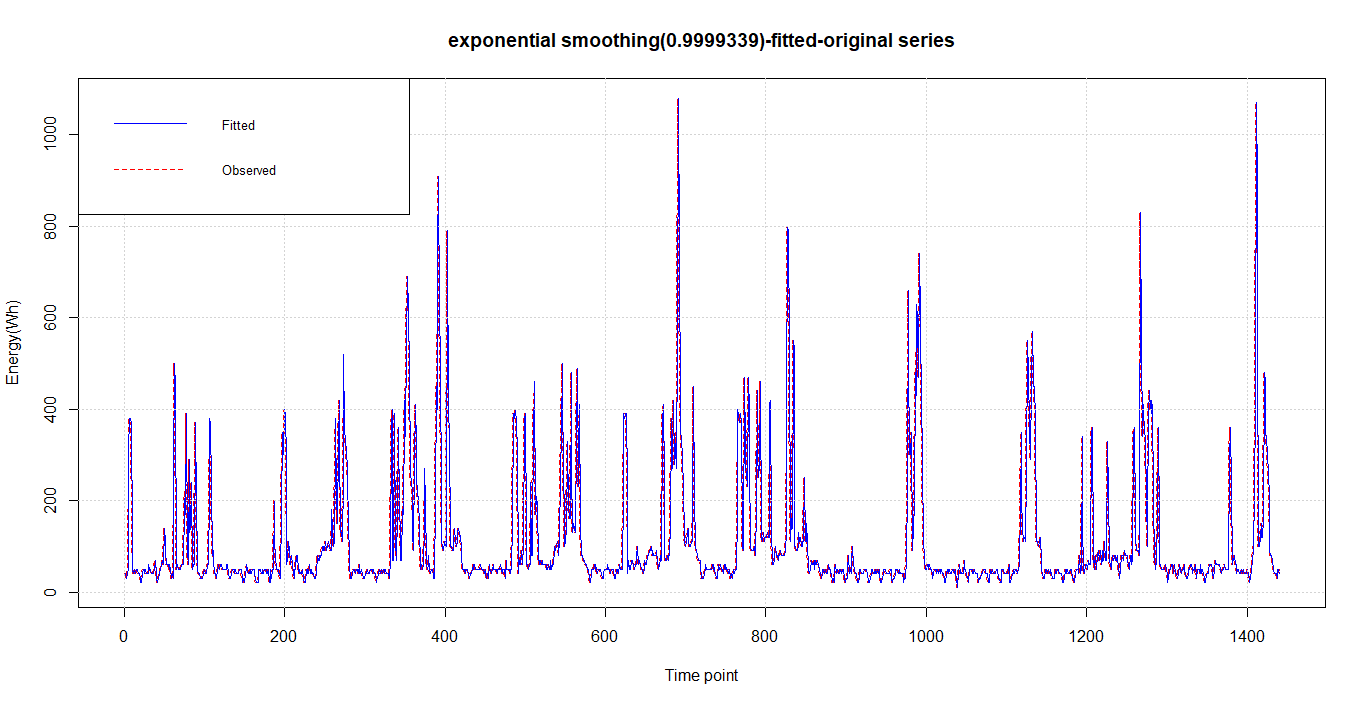
\includegraphics[width=\linewidth]{figure19-1.png}
  \end{subfigure}
  \begin{subfigure}[b]{0.6\linewidth}
    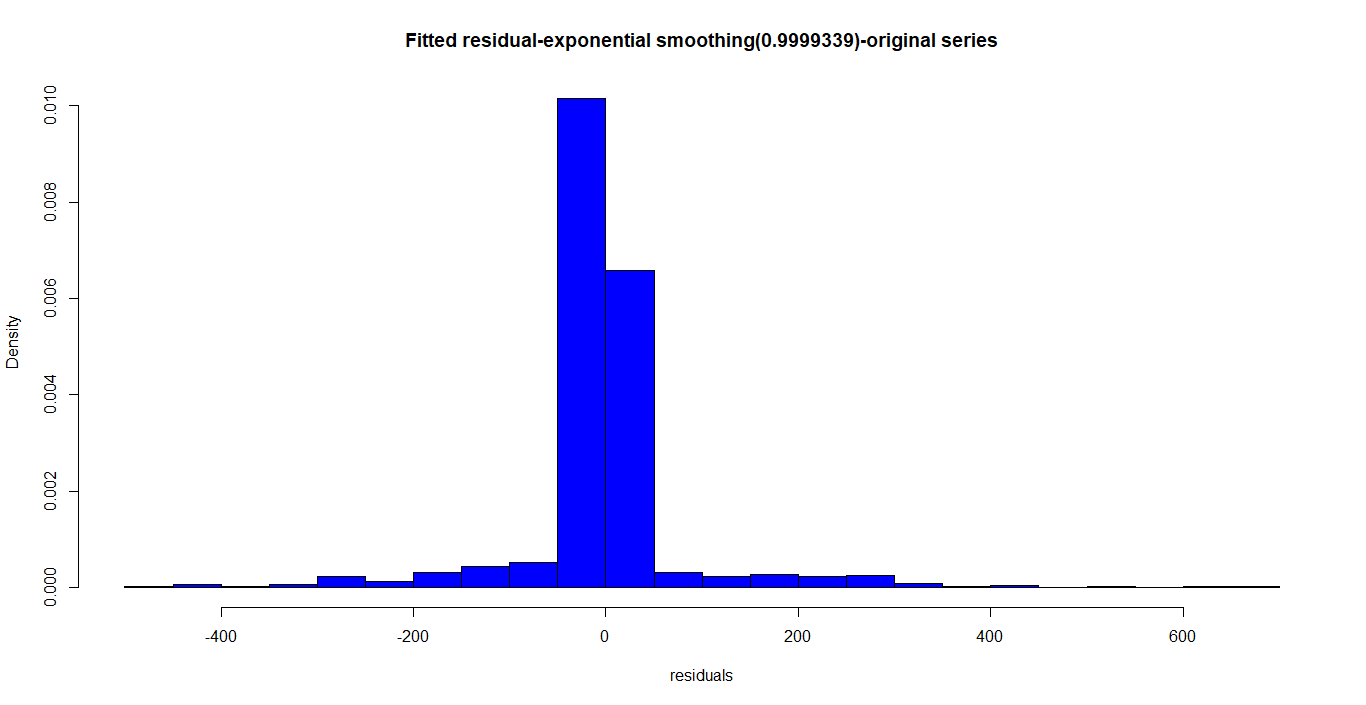
\includegraphics[width=\linewidth]{figure19-2.png}
  \end{subfigure}
  \begin{subfigure}[b]{0.6\linewidth}
    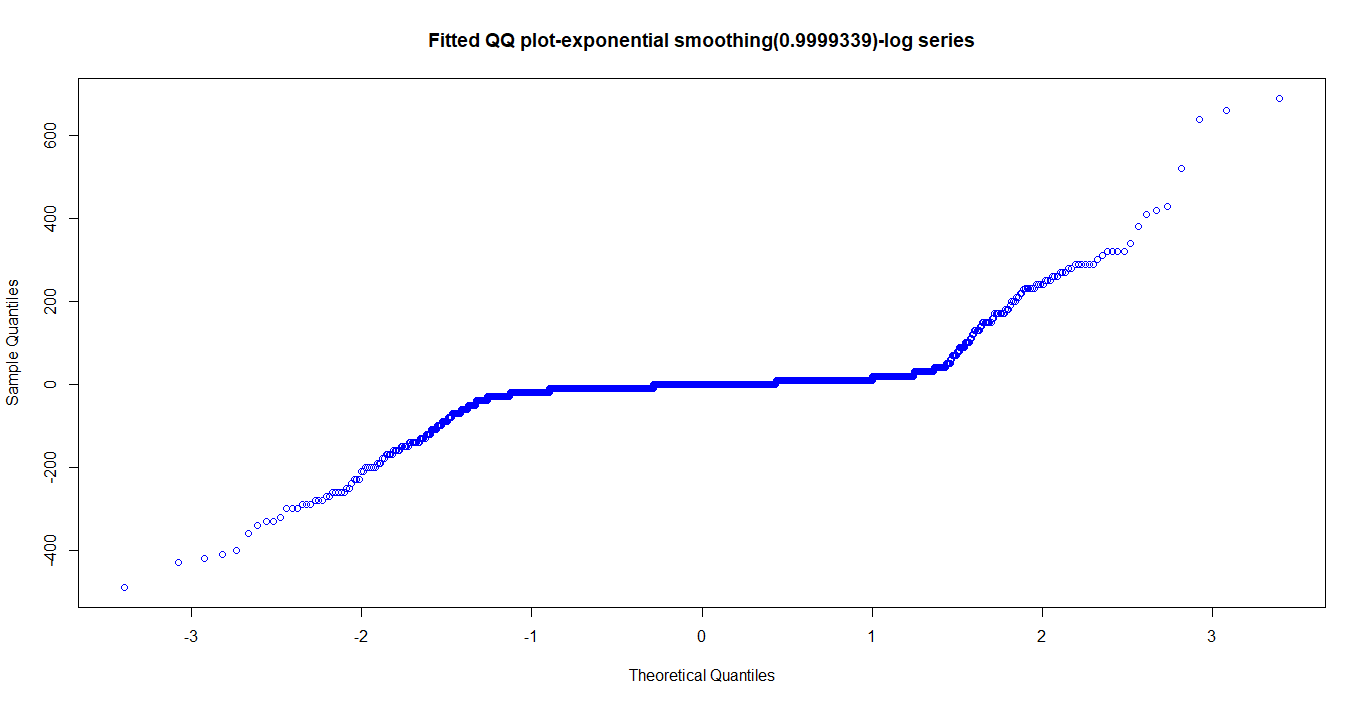
\includegraphics[width=\linewidth]{figure19-3.png}
  \end{subfigure}
  \begin{subfigure}[b]{0.6\linewidth}
    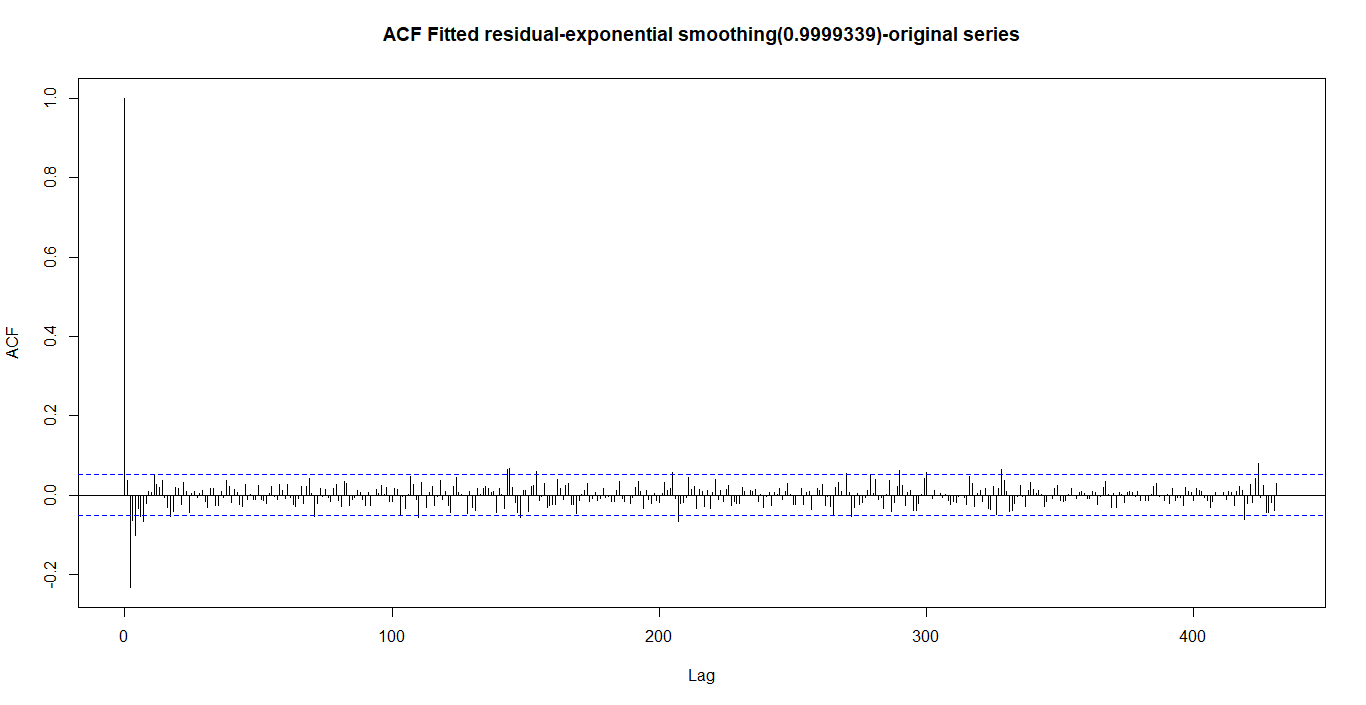
\includegraphics[width=\linewidth]{figure19-4.png}
  \end{subfigure}
  \caption{Exponential Smoothing ($\alpha=0.9999339$)}
  \label{fig:figure19}
\end{figure}

\paragraph{}
The histogram does not show the normal shape. Interestingly, it shows that the residual values quite centralized around zero, indicating that the algorithmm fits quite well the observed data. The acf of the residuals also looks quite nice since there are no clear patterns. Here is the forecast of the algorithm.
\begin{figure}[H]
  \centering
  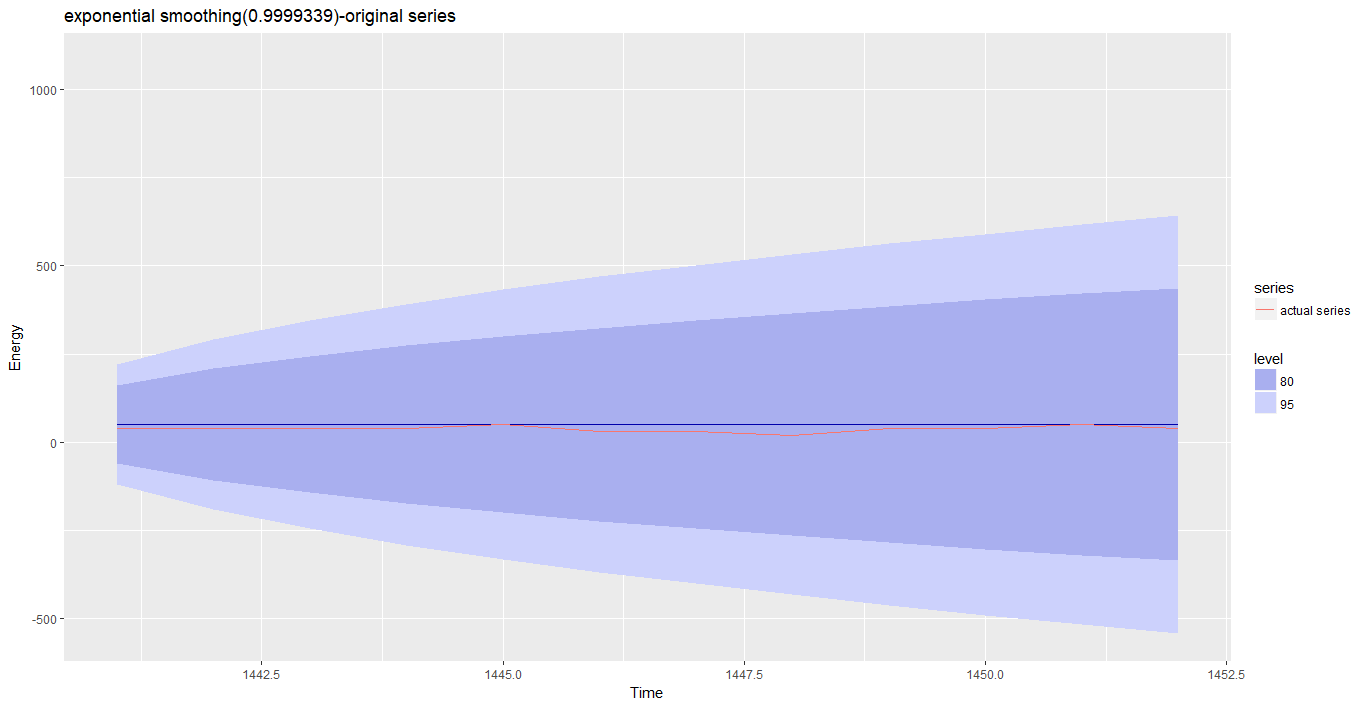
\includegraphics[width=\linewidth]{figure19-5.png}
  \caption{Exponential Smoothing ($\alpha=0.9999339$) - Forecast}
  \label{fig:figure20}
\end{figure}

\paragraph{}
The forecast seems to be naive, failing to catch no variation in the series, although it shows to be quite closed to the original values. This could be because from the point when there is no observed value left, the algorithm takes on the previously predicted value to applied for the forecast, meaning $F_{t+1}=F_t+\alpha(y_t-F_t)=F_t +\alpha(F_t-F_t)=F_t$ in which $t$ is the out of sample point of time. Fortunately in this case, the series didn't have any large variation.

\paragraph{}
Next, the same approach is used for the Holt's linear algorithm. This algorithm is an extension of the exponential smoothing algorithm. It incorperates a term for linear trends. There are two parameters to be observed. The following plots show how each of the parameters affect the performance of the model.
\begin{figure}[H]
  \centering
  \begin{subfigure}[b]{1\linewidth}
    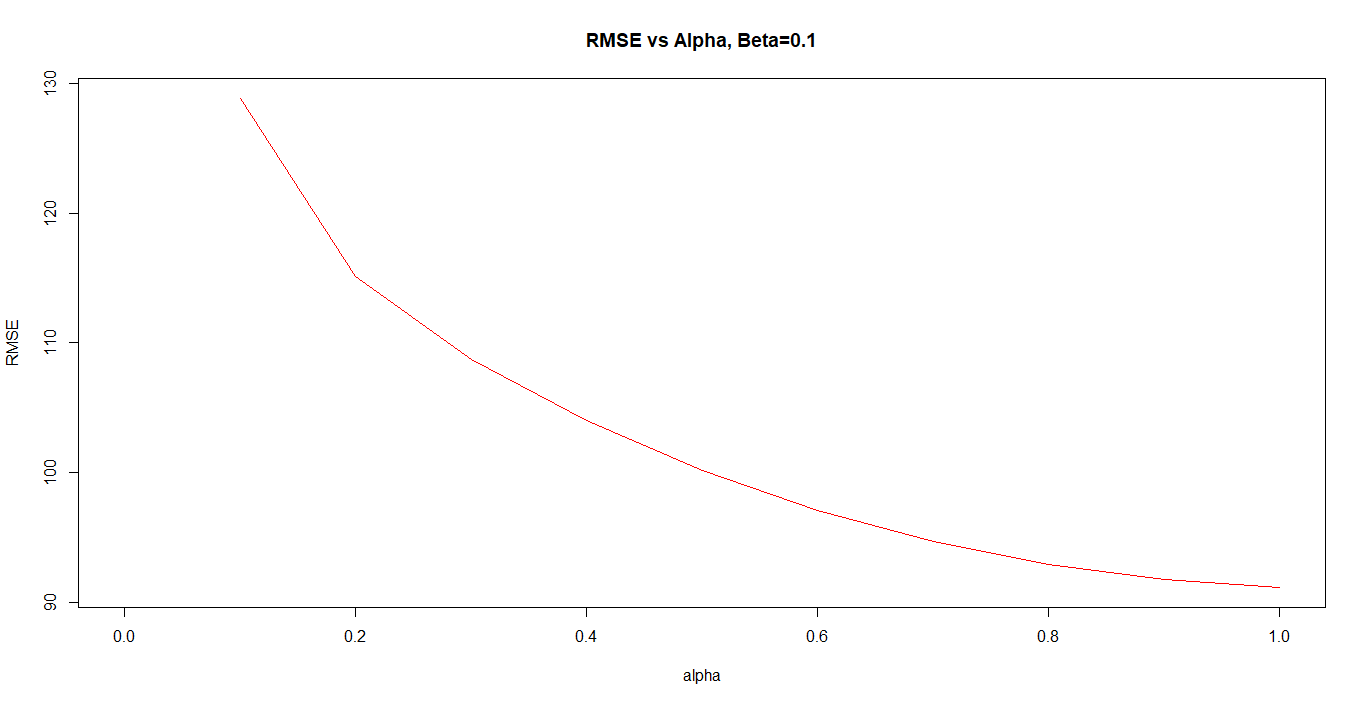
\includegraphics[width=\linewidth]{figure20-1.png}
  \end{subfigure}
  \begin{subfigure}[b]{1\linewidth}
    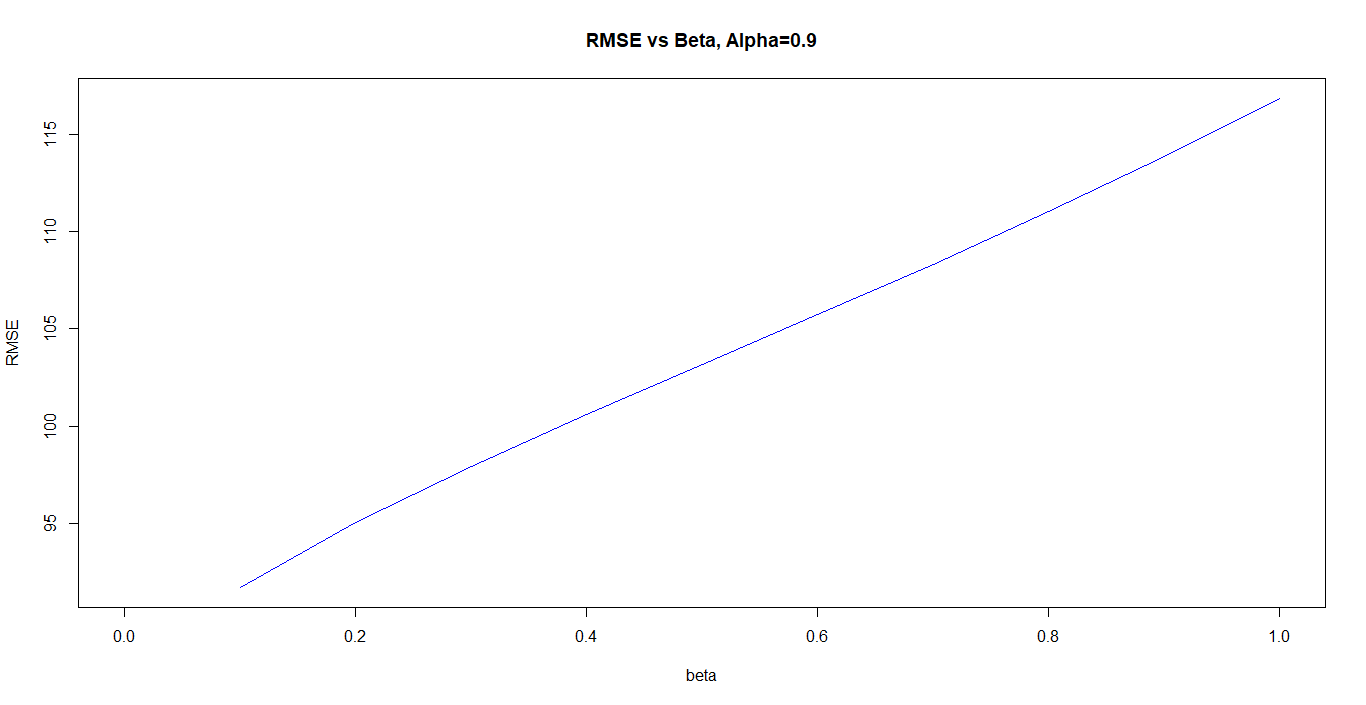
\includegraphics[width=\linewidth]{figure20-2.png}
  \end{subfigure}
  \caption{The effects of $\alpha$ and $\beta$}
  \label{fig:figure21}
\end{figure}

\paragraph{}
As can be seen, increasing $\alpha$ could reduce the RMSE, meanwhile the opposite happens to $\beta$. The optimal value of $\alpha$ is expected to be close to 1 and that of $\beta$ is expected to be close to 0. Using R package, the optimal model is obtained. The model is Holt's linear($\alpha=1$, $\beta=0.01253426$). This model is applied on the \textbf{log series}, since R gives a warning message regarding the difficulty in optimization when using the original series. Figure ~\ref{fig:figure22} shows the results of the model on the log series
\begin{figure}[H]
  \centering
  \begin{subfigure}[b]{0.6\linewidth}
    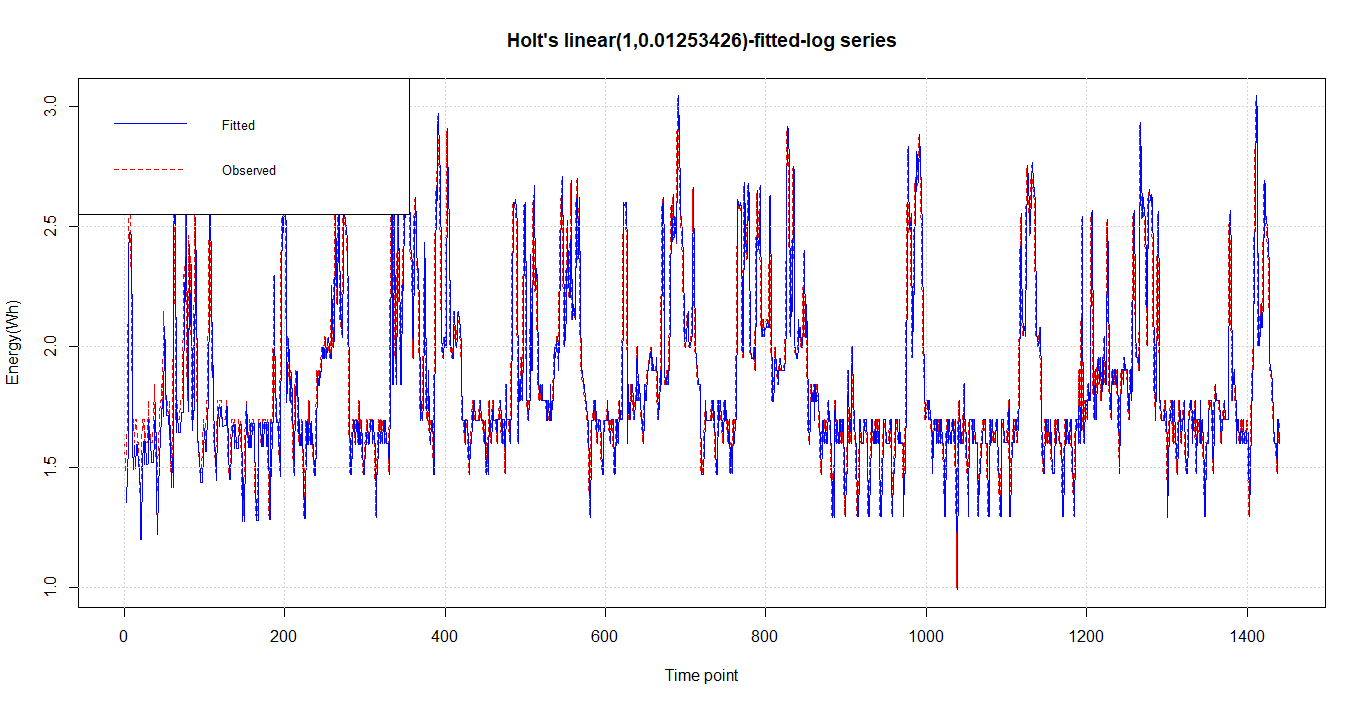
\includegraphics[width=\linewidth]{figure21-1.png}
  \end{subfigure}
  \begin{subfigure}[b]{0.6\linewidth}
    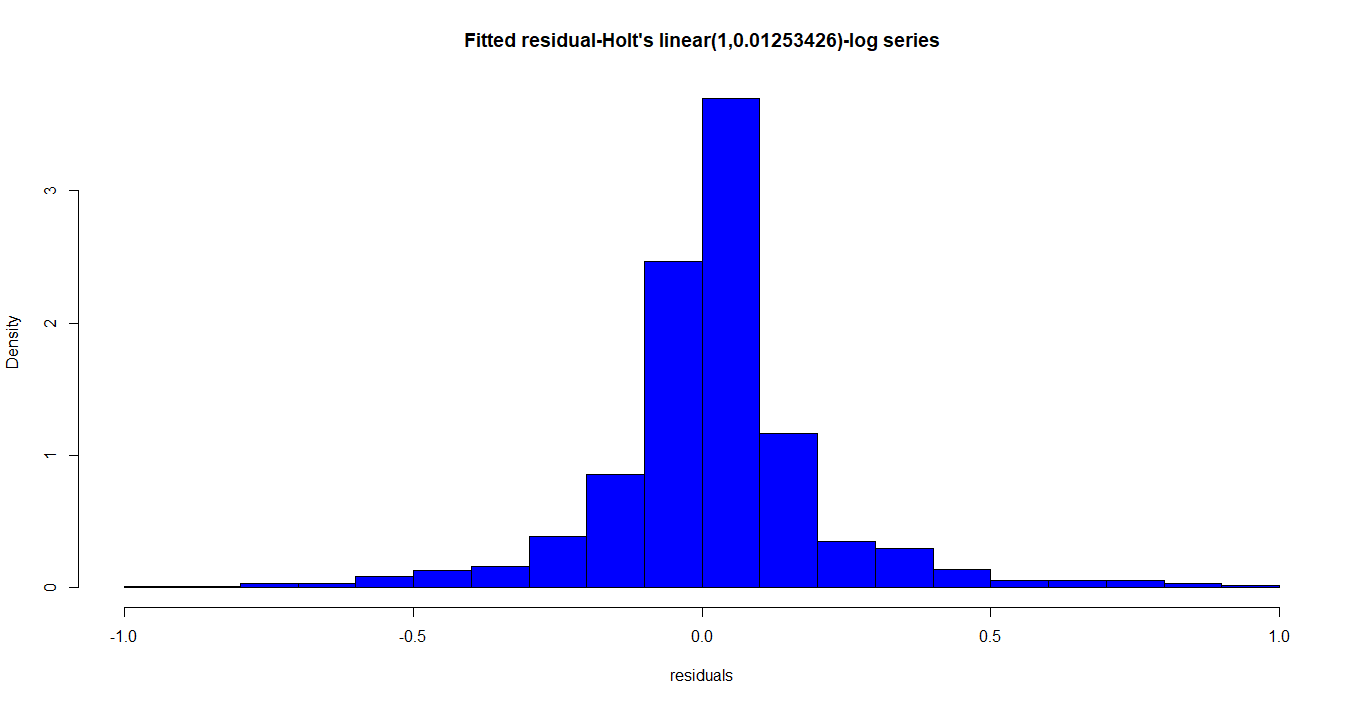
\includegraphics[width=\linewidth]{figure21-2.png}
  \end{subfigure}
  \begin{subfigure}[b]{0.6\linewidth}
    \includegraphics[width=\linewidth]{figure21-3.png}
  \end{subfigure}
  \begin{subfigure}[b]{0.6\linewidth}
    \includegraphics[width=\linewidth]{figure21-4.png}
  \end{subfigure}
  \begin{subfigure}[b]{0.6\linewidth}
    \includegraphics[width=\linewidth]{figure21-5.png}
  \end{subfigure}
  \begin{subfigure}[b]{0.6\linewidth}
    \includegraphics[width=\linewidth]{figure21-6.png}
  \end{subfigure}
  \caption{Holt's linear($\alpha=1$, $\beta=0.01253426$)}
  \label{fig:figure22}
\end{figure}

\paragraph{}
The model shows to have similar results as previous ones. No significant improvements are obvious. However, there is a slight trend in the forecast in opposed to projecting a straight line into the future.

\paragraph{}
The final algorithm in this group to be applied is the Additive Holt Winter algorithm, which contains a seasonal component. The similar approach is done and below shows the effect of each parameter.
\begin{figure}[H]
  \centering
  \includegraphics[width=\linewidth]{figure22.png}
  \caption{The effects of $\alpha, \beta$ and $\gamma$}
  \label{fig:figure23}
\end{figure}

\paragraph{}
The figure show how each parameter impacts on the RMSE. As can be seen, the optimal values for $\alpha, \beta, \gamma$ could be around 0.8, 0.1 and 0.8 respectively. Using R package, the returned parameters are $\alpha=0.8,\beta=0,\gamma=1$, which is close to the expectation. Figure ~\ref{fig:figure24} shows the results of the model on the log series.
\begin{figure}[H]
  \centering
  \begin{subfigure}[b]{0.6\linewidth}
    \includegraphics[width=\linewidth]{figure23-1.png}
  \end{subfigure}
  \begin{subfigure}[b]{0.6\linewidth}
    \includegraphics[width=\linewidth]{figure23-2.png}
  \end{subfigure}
  \begin{subfigure}[b]{0.6\linewidth}
    \includegraphics[width=\linewidth]{figure23-3.png}
  \end{subfigure}
  \begin{subfigure}[b]{0.6\linewidth}
    \includegraphics[width=\linewidth]{figure23-4.png}
  \end{subfigure}
  \begin{subfigure}[b]{1\linewidth}
    \includegraphics[width=\linewidth]{figure23-5.png}
  \end{subfigure}
  \caption{Holt Winter( $\alpha=0.8,\beta=0,\gamma=1$)}
  \label{fig:figure24}
\end{figure}

\paragraph{}
Although the forecast of given by the parameters are quite good, the fit is not adequate. The acf plot show quite high autocorrelation in the residuals. Carefully check the panel on the top left, one can see that at some points the evergy receives negative values. The following table summarizes the MAPE values of the algorithms computed in the original scale. 
\begin{table}[H]
  \begin{center}
    \caption{MAPE}
    \label{tab:table4}
    \begin{tabular}{l|S|S} % <-- Alignments, all center
      \textbf{Model} & \textbf{MAPE} &  \textbf{Test MAPE}\\
      \hline
  Exp. Smoothing(0.9999339)&0.3036788&0.3819306\\
  Holt's linear(1,0.01253426)&0.3078541&0.3502281\\
  HoltWinter(0.8,0,1)&0.6217661&0.5378387\\
    \end{tabular}
  \end{center}
\end{table}

\paragraph{}
As the table suggests, one should opt to Holt's linear algorithm in this case since it gives the lowest test MAPE. However, the Holt Winter is also worth considering because the algorithm takes into the seasonality components. 

\subsection{Models that can deal with changing variance over time}
\paragraph{}
As the original series shows to have unstable variance over time, it is worth considering a model that can cope with changing variance. In this section, we attempt to see if a GARCH model could do a better job for the problem. We first conduct some analysis to make sure that the method fits the series. The series is first transformed into log scale, then the first order difference at lag 1 is taken. Let the resulting series be called $x_t$. Here is how $x_t$ looks like.
\begin{figure}[H]
  \centering
  \includegraphics[width=\linewidth]{figure24.png}
  \caption{$x_t$ series}
  \label{fig:figure25}
\end{figure}

\paragraph{}
The series looks like it is stationary in mean, the variance, however, is not. This can be checked by the acf plots of the $x_t$ series and the $x_t^2$ series, which represents the variance.
\begin{figure}[H]
  \centering
  \includegraphics[width=\linewidth]{figure25.png}
  \caption{$x_t$ series}
  \label{fig:figure26}
\end{figure}

\paragraph{}
The acf of the $x_t$ series goes to zero quickly, meanwhile, the acf of the $x_t^2$ series show somes patterns, showing evidence against stationary. This fits the description of a series where a GARCH model may be suitable. Alternatively, GARCH(1,1)-ARMA(1,1) is applied to the original series to avoid having to transform and undifferencing the series. Figure ~\ref{fig:figure27} shows the learned model. 
\begin{figure}[H]
  \centering
  \includegraphics[width=0.5\linewidth]{figure26.png}
  \caption{acf of $x_t$ and $x_t^2$}
  \label{fig:figure27}
\end{figure}

\paragraph{}
Notice that the p-values of the coefficients are all very small, indicating they are statistically significant. Figure ~\ref{fig:figure28} shows the results.
\begin{figure}[H]
  \centering
  \begin{subfigure}[b]{0.6\linewidth}
    \includegraphics[width=\linewidth]{figure27-1.png}
  \end{subfigure}
  \begin{subfigure}[b]{0.6\linewidth}
    \includegraphics[width=\linewidth]{figure27-2.png}
  \end{subfigure}
  \begin{subfigure}[b]{0.6\linewidth}
    \includegraphics[width=\linewidth]{figure27-3.png}
  \end{subfigure}
  \begin{subfigure}[b]{0.6\linewidth}
    \includegraphics[width=\linewidth]{figure27-4.png}
  \end{subfigure}
  \caption{GARCH(1,1)-ARMA(1,1)}
  \label{fig:figure28}
\end{figure}

\paragraph{}
The results are similar to previous models. The errors are assumed to follow a normal distribution with mean 0 and variance changing over time, therefore the histogram of the errors and the QQ plot should looks different than those of a sample drawn from a normal distributtion.The acf plot of the residuals is quite nice, although some lag still has high autocorrelation. When using a GARCH component to model the error, the forecasts for the series and the sigma series are of interests. The R package for forecasting provide two different modes: the k-step ahead standard forecast and the rolling forecast. The standard forecast will be based on the unconditional expectation of the model. The rolling forecast give the model the ability to update the forecast once a new data point is observed. This requires the out-of-sample setting. The number of rolling forecast must not be greater than the number of out-of-sample data points. Figure ~\ref{fig:figure29} shows forecasts of the model.
\begin{figure}[H]
  \centering
  \begin{subfigure}[b]{0.6\linewidth}
    \includegraphics[width=\linewidth]{figure28-1.png}
  \end{subfigure}
  \begin{subfigure}[b]{0.6\linewidth}
    \includegraphics[width=\linewidth]{figure28-2.png}
  \end{subfigure}
  \begin{subfigure}[b]{0.6\linewidth}
    \includegraphics[width=\linewidth]{figure28-3.png}
  \end{subfigure}
  \begin{subfigure}[b]{0.6\linewidth}
    \includegraphics[width=\linewidth]{figure28-4.png}
  \end{subfigure}
  \caption{The top panels show the standard forecasts and the rolling forecasts for the series. The lower panels show the standard forecasts and the rolling forecasts for the sigma series.}
  \label{fig:figure29}
\end{figure}

\paragraph{}
The rolling forecasts clearly does a better job, since the forecasts does not seem to be naive, it could be because they get updated on each rolling basis. In the lower left panel, the volatility is expected to increase in the next 12 steps, meanwhile it is shown to be level in the lower left panel, which is made by the rolling forecast approach and is actually more correct. 

\paragraph{}
Notice that this is not the best order sets for this approach. To choose the best fit order of the models, optimization must be done against some measures such as RMSE or AIC. Within the scope of this project, the optimization is not presented here. The fitted MAPE and the test MAPE of the model is 0.3157198 and 0.5724684 respectively, calculated based on the rolling forecasts. The AIC of the model is 10.954. However, we cannot compare this value with previous model since the AIC given by the package is defined differently as follow:
\begin{equation*}
  \centering
AIC=\frac{1}{N}(-2LogLikelihood+2m)
\end{equation*}
\begin{itemize}
  \item $N$ is the number of data points
  \item $m$ is the number of fitted parameters
\end{itemize}

\section{Results and conclusion}
\paragraph{}
The following table summarizes the results of the fitted models.
\begin{table}[H]
  \begin{center}
    \caption{Summary}
    \label{tab:table5}
    \begin{tabular}{l|S|S} % <-- Alignments, all center
      \textbf{Model} & \textbf{Test MAPE} &  \textbf{AIC}\\
      \hline
  AR(1) &0.3923939  &-664.2\\
  AR(3) &0.3926326  &-714.86\\
  MA(1) &0.3974313  &-664.92\\
  MA(3) &0.3701166  &-747.59\\
  ARIMA(1,0,1)(1,1,1)[144]  &0.8108953  &-458.34\\
  ARMA(3,3) &0.6669242  &-803.36\\
  Exp. Smoothing (0.9999339)  &0.3819306  &x\\
  Holt's linear(1,0.01253426) &0.3502281  &x\\
  HoltWinter(0.8,0,1)  &0.5378387 &x\\
  GARCH(1,1)-ARMA(1,1)  &0.5724684  &10.954*\\
    \end{tabular}
  \end{center}
\end{table}

\paragraph{}
The MAPE in these section is computed on the original series for consistency in comparison. However, the AIC in the GARCH model is computed by a different formula as mentioned before. If using the test MAPE as the criteria of choosing the model, one would opt to Holt's linear since the model gain the lowest test MAPE value. However, observing the Figure ~\ref{fig:figure3} again we notice one important thing that we have not taken into account: The energy consumption at the end of a day and at the beginning of a day are usually low and stable, slightly fluctuating around 40 to 50. Since we take a sample of 10 days of data to fit the model, and then try to make forecast for the next two hours (12 data points), therefore, it does not show a big difference between models which do not take into account seasonality and variation and models which do so. As one can see here, some models such as MA(3), Holt's linear or AR(3) recieve quite good results, meanwhile GARCH, which can deal with changing variance, seems not to have an ideal test MAPE. However, the next question is: If we had sampled at different periods where variance is high, how would these models have performed? To answer this question, further investigation needs to be done. Here, we show a small experiment to illustrate this idea.
\paragraph{}
The following figure shows the forecasts of the GARCH model and the Holt's linear algorithm on a different period. The fitting procedure is the same, however, the period is intendedly chosen to have high variation in the forecast set.  
\begin{figure}[H]
  \centering
  \begin{subfigure}[b]{1\linewidth}
    \includegraphics[width=\linewidth]{figure29-1.png}
  \end{subfigure}
  \begin{subfigure}[b]{1\linewidth}
    \includegraphics[width=\linewidth]{figure29-2.png}
  \end{subfigure}
  \caption{GARCH and Holt's linear forecasts on original series}
  \label{fig:figure30}

\end{figure}
\paragraph{}
Clearly that the Holt's linear completely failed to capture the variation in the series, on the other hand the GARCH shows to do a better job. Due to this reason, we would lean towards models that could capture seasonality and variation such as GARCH and try to optimize the parameters of the model to get the best result in the near future experiments.
\end{document}
